\documentclass[11pt]{article}
\usepackage{fullpage}
\usepackage{algorithmic}
\usepackage{algorithm}
\usepackage{epsfig}
\usepackage{epstopdf}
\usepackage{graphicx}
\usepackage{latexsym}
\usepackage{amsmath}
\usepackage{amsfonts}
\usepackage{multirow}
\usepackage{amssymb}
\DeclareMathOperator*{\argmax}{argmax}
\DeclareMathOperator*{\dis}{dis}
\usepackage{mathrsfs}
%\usepackage[mathcal]{eucal}
\usepackage{pifont}
\usepackage{yhmath}
\usepackage{undertilde}
\usepackage{bbm}
\usepackage{bm}
%\usepackage{dsfont}
\usepackage{eufrak}
\usepackage{amsthm}
\usepackage{booktabs}
\usepackage[usenames,dvipsnames]{color}
%\usepackage[usenames]{color}
\usepackage{stmaryrd}
\usepackage{wasysym}
\usepackage{bbm}
\usepackage{array}
\usepackage{enumerate}
%\usepackage[ruled]{algorithm2e}
%\renewcommand{\algorithmcfname}{ALGORITHM}

\bibliographystyle{plain}

%\newtheorem{algorithm}{Algorithm}
\newtheorem{mechanism}{Mechanism}
\newtheorem{theorem}{Theorem}[section]
\newtheorem{lemma}[theorem]{Lemma}
\newtheorem{property}[theorem]{Property}
\newtheorem{claim}[theorem]{Claim}
\newtheorem{corollary}[theorem]{Corollary}
\newtheorem{proposition}[theorem]{Proposition}
\newtheorem{definition}[theorem]{Definition}
\newtheorem{remark}[theorem]{Remark}
\newtheorem{conjecture}[theorem]{Conjecture}
%\newtheorem{algorithm}{Algorithm}[section]
\newtheorem{hypothesis}[theorem]{Hypothesis}
\newtheorem{observation}[theorem]{Observation}

\theoremstyle{remark}
\newtheorem{problem}[theorem]{Problem}
\newtheorem{example}[theorem]{Example}
%\newtheorem{procedure}{Procedure}
\newtheorem{assumption}{Assumption}
%\newtheorem{claim}{Property}

\def\bfm#1{\mbox{\boldmath$#1$}}
 \newcommand{\qedd}{\hfill\rule{1 ex}{1 ex}}

\makeatletter
\newcommand\figcaption{\def\@captype{figure}\caption}
\newcommand\tabcaption{\def\@captype{table}\caption}
\makeatother

\newcommand{\comment}[1]{\textcolor{black}{\textrm{#1}}}
\newcommand{\rrcomment}[1]{\textcolor{red}{\textbf{#1}}}
\newcommand{\bluecomment}[1]{\textcolor{blue}{\textrm{#1}}}
\newcommand{\greencomment}[1]{\textcolor{OliveGreen}{\textrm{#1}}}
\newcommand{\redcomment}[1]{\textcolor{red}{\textrm{#1}}}
\newcommand{\ma}[1]{\textcolor{magenta}{\textrm{#1}}}

\newcommand{\med}{\text{med}}
\newcommand{\msc}[1]{\ensuremath{\text{\sc #1}}\xspace}
\newcommand{\st}{\msc{st}}
\newcommand{\opt}{\msc{opt}}

\DeclareMathAlphabet{\mathpzc}{OT1}{pzc}{m}{it}

\begin{document}
\newcounter{my}
\newenvironment{mylabel}
{
\begin{list}{(\roman{my})}{
\setlength{\parsep}{-1mm}
\setlength{\labelwidth}{8mm}
\usecounter{my}}
}{\end{list}}

\newcounter{my2}
\newenvironment{mylabel2}
{
\begin{list}{(\alph{my2})}{
\setlength{\parsep}{-0mm} \setlength{\labelwidth}{8mm}
\setlength{\leftmargin}{3mm}
\usecounter{my2}}
}{\end{list}}

\newcounter{my3}
\newenvironment{mylabel3}
{
\begin{list}{(\alph{my3})}{
\setlength{\parsep}{-1mm}
\setlength{\labelwidth}{8mm}
\setlength{\leftmargin}{10mm}
\usecounter{my3}}
}{\end{list}}

\title{Social Choice for Eliminating the Worst Candidate\\ under Metric Preferences}

\vspace{-6em}

\maketitle

\vspace{-3em}

\begin{center}\large

\author{Jianan Lin (jnlin16@fudan.edu.cn),\\ Chenhao Wang (chenhwang4-c@my.cityu.edu.hk)}

\end{center}

\vspace{2em}

%\vspace{2em}

\begin{abstract}
We consider social choice rules under the metric preferences: both voters and candidates are points in a metric space, and each voter prefers candidates that are closer to her to ones that are further away. We study the problem of selecting the least popular candidate to eliminate. Each voter takes the distance to the eliminated one as her utility, and the objective is to maximize the total utility of all voters.  The underlying distances can be arbitrary, implicit, and unknown. Based only on the voters' preference rankings that are consistent with the metric distances, a social choice rule may not identify an optimal candidate. The quality of a rule is measured by its distortion, defined as the worst-case ratio between the performance of an optimal candidate and that of the selected one. We present a social choice rule with distortion of 4.236, using a symmetric idea of the Weighted Uncovered rule. Further, we design a new rule with improved distortion of 3.828 for a subclass of instances, including all instances with no more than 6 candidates. Both rules only look at the weighted tournament graph on the candidates. We also contribute to the well-studied problem of selecting a candidate to minimize the total distance to all voters, improving the distortion to 3.828 when there are no more than 6 candidates.
%For the social cost objective, it is desirable to select a candidate as winner that minimizes the sum of distances to the voters, and each voter takes the distance to the winner as her cost.

 \noindent{\bf Keywords:} Social choice; Metric preferences; Distortion
\end{abstract}

%optimal auctions, bilateral trade, sequential auctions, online algorithms, competitive analysis


\section{Introduction}

In social choice theory, a \emph{mechanism} (also referred to as a voting rule or a social choice rule) aggregates the preferences of multiple voters over a set of candidates, and returns  a candidate as the winner of the election. The preference of a voter is often represented as a linear order over the candidates. There is no consensus on what are the best voting rules, and most of the social choice literature compares different voting rules by defining normative or axiomatic criteria, such as anonymity, neutrality and Pareto efficiency.

An appealing approach to dealing with social choice problems is embedding the input ``election'' into a \emph{metric space}, \emph{i.e.}, each participant is represented by a point in a metric space, and voters %tend to
prefer candidates that are closer to them to the ones that are further away. This spatial model has very natural interpretations. For example, in a 2-dimensional Euclidean space, each dimension specifies a political issue (such as military or education), and the position of a voter or candidate identifies the extent to which the individual supports the issues. Recently, this model has attracted attentions from AI researchers, see, {\em e.g.,} \cite{anshelevich2015approximating,elkind2017multiwinner,abramowitz2019awareness}.


 As voters' preferences are specified by their distances to candidates,  it is natural to quantify the {\em quality} of the selected candidate by the associated distances. %the sum of its distances to all voters. We aim at selecting a committee that optimizes (minimizes or maximizes) this objective function.
  We evaluate the  performance of a mechanism in the standard worst-case analysis benchmark (introduced by Procaccia and Rosenschein \cite{procaccia2006distortion}), which defines the \emph{distortion} of a mechanism to be the worst-case ratio between the quality of an alternative selected by this mechanism and that of the optimal alternative selected by an omniscient mechanism. More generally, the distortion, which stems from an information deficiency, is a measure of how close it always gets to the optimal alternative.

   Previous works were mainly concerned about the single-winner election that aims to select one candidate, minimizing the total distance to all voters. In this paper, we focus on the antithesis, the \emph{single-loser} election that aims to select one candidate, maximizing the total distance to all voters. That is, we want to eliminate the least popular candidate. When the context is clear, the selected candidate is also called the winner of the election, even though this is more like a ``loser". Every voter wants to stay as far away as possible from this winner.
This election is well motivated, for example, some enterprises adopt a \emph{last-out} mechanism in the personnel performance appraisal system, which dismisses the employee with the lowest performance in a department each year. %some voting rules in government policy and TV talent shows iteratively eliminate one candidate at each time to obtain the final winners.
Besides, a voting rule for the single-loser election may be iteratively used as a subroutine for multi-winner elections in  TV talent shows, eliminating one candidate at each iteration.

 %Previous work mainly concerned about the social cost objective, providing distortion bounds for scv mechanisms in single-winner elections and \emph{ranking} mechanisms that ask for linear orders as input. In this paper, we bound the distortion for scv mechanisms in multi-winner elections w.r.t. social cost, and scv mechanisms in single-winner elections w.r.t. social utility.

\medskip\noindent\textbf{Our Results and Organizations}

We consider the social choice problem under metric preferences, in which all participants are assumed to be points in a metric space, and the preferences are identified by the distances. The commonly studied objective is to minimize the total distance of the selected candidate to all voters, called the social cost objective.
In this work, we study the social choice rules for the problem of selecting a candidate with maximum total distance to all voters. As it is  only given the ordinal preference orderings, instead of the underlying metric costs which generate these preferences, a rule cannot always select the optimal candidate. We measure the performance of a social choice rule by its distortion, defined as the worst-case ratio between the social value of the optimal candidate and the one returned by the rule.

%In other words, we show how closely social choice functions approximate the optimal alternative when they are given only the ordinal preference orderings, instead of the underlying metric costs which generate these preferences.

Section \ref{sec:pre} gives the preliminaries. Assume each voter takes the distance to the selected candidate as her utility, and the \emph{social utility} is the sum of all voters' utilities. In this work we consider the problem of maximizing the social utility. Several typical voting rules for the social cost objective in the literatures (e.g., Weighted Uncovered in \cite{munagala2019improved}) are presented: some of them can be applied to our problem with the same distortion, by reversing the input preference orders.

In Section \ref{sec:max}, we provide two lemmas that bound the ratio between the social utilities of two candidates. They are the key tools for analysis throughout this paper. Then we adapt the Weighted Uncovered rule for the social utility objective: it selects a candidate $A$ such that for any other candidate $B$, either at least $z$ fraction of voters prefer $B$ to $A$, or there exists a candidate $C$ such that at least $1-z$ fraction prefers $C$ to $A$ and at least $z$ fraction prefers $B$ to $C$. By setting an appropriate parameter $z$, we obtain a voting rule with distortion 4.236 (proved by using the lemmas), the same with that of Weighted Uncovered for the social cost version.


In Section \ref{sec:im}, the power of the two lemmas can be used to improve the distortion for a subclass of instances. We propose a voting rule that selects a candidate arbitrarily from a (possibly empty) set, called $Cov_{su}$-set, only based on the fraction of voters who prefer $A$ to $B$, for each pair of candidates $A,B$. Setting an appropriate parameter, we prove that this rule achieves a distortion 3.828 if the $Cov_{su}$-set is non-empty. Although we are not able to identify when this set is empty in general, we prove that this set contains at least one candidate for a subclass of instances, including all instances with no more than 6 candidates. Hence, we improve the distortion from 4.236 to 3.828 for such a subclass, and leave the application range of this rule as an open question.

%For the special case with only 3 candidates, Munagala and Wang \cite{munagala2019improved} proved that a rule called MatchingUncovered has a distortion 3, which computes a perfect matching in a constructed bipartite graph. We show that a much simpler rule can also achieve a distortion 3:  marking each vertex in the weighted tournament graph, with a number equal to the weight of the edge with the least weight from this point, and selecting the vertex with maximum mark.

In Section \ref{sec:min} we extend the results in Section \ref{sec:im} to the well-studied problem for social cost objective, and provide improved distortion 3.828 when there are 5 or 6 candidates (the best known distortion is 4.236 by Weighted Uncovered).  Section \ref{sec:dis} discusses egalitarian objectives and concludes this paper.



\medskip\noindent\textbf{Related Work}

In social choice theory, Procaccia and Rosenschein \cite{procaccia2006distortion} propose a utilitarian approach -- the implicit utilitarian voting -- by assuming that voters have latent cardinal utilities and report ordinal preferences induced by them. They measure the performance of popular voting rules by the notion of \emph{distortion}. Subsequently, Caragiannis and Procaccia \cite{caragiannis2011voting}, Oren and Lucier \cite{oren2014online}, Boutilier \emph{et al.} \cite{boutilier2015optimal}, Bhaskar and
Ghosh \cite{bhaskar} employ this notion and design selection rules with low distortions.

Anshelevich \emph{et al.} \cite{anshelevich2015approximating} first embed the social choice into a metric space, in which the participants are points, and the
costs are driven by the distances. For the social cost objective of selecting a candidate to minimize the total distance to all voters, they show that the uncovered set rules \cite{moulin1986choosing} (including the Copeland rule) can guarantee distortion at most 5. They also prove that any deterministic rule has a lower bound for distortion of at least 3. Later, Skowron and Elkind \cite{skowron2017social} show that the class of scoring rules and STV have super-constant distortion. %A weighted tournament graph means placing two opposite directed edges between two candidates with weight equal to the rate of voters who prefer the first candidate to the total number of voters.
 Goel \emph{et al.} \cite{gross2017vote} show the ranked pairs rule and the Schulze method working on weighted tournament graph on the candidates both have distortion of at least 5. Recently, Munagala and Wang  \cite{munagala2019improved} propose a Weighted Uncovered rule with distortion $2+\sqrt5\approx 4.236$. They additionally give a conjecture that the perfect matching rule can always guarantee a distortion at most 3, matching the lower bound. All above mentioned rules are deterministic and work for the social cost objective.


Randomized social choice rules  have also been studied in the metric distortion setting, which output a probability distribution over the set of candidates. The lower bound on distortion of randomized rules is 2 \cite{anshelevich2017randomized} \cite{feldman2016voting}. Random dictatorship that randomly selects
the top choice of one of the $m$ voters gets distortion $3-2/m$ \cite{anshelevich2017randomized} \cite{feldman2016voting}. Gross \emph{et al.} \cite{gross2017vote}
 propose a simple mechanism that randomly asks voters for their top choice until two voters agree, achieving very low distortion when the number of candidates is not large.
However, randomized social choice rules attract less attention than deterministic ones in practise.

 Some works focus on other objectives or properties. The work of Anshelevich et al. \cite{anshelevich2015approximating} considers the objective of minimizing the median cost of agents, and proves that the Copeland rule achieves  the optimal distortion of 5. Fairness property is also considered \cite{goel2018relating} \cite{munagala2019improved}.

 %the quality of a candidate is defined as the median of agent costs for that candidate: this captures the objective that the best candidate is the one which minimizes the cost of the median voter, instead of the average voter.


%Our other objective function defines the quality of an alternative as the median of agent costs for that alternative: this captures the objective that the best alternative is the one in which the cost of the median voter is minimized, instead of the average voter.

\emph{Other problems.} Some works study other social choice problems in the metric distortion setting. When candidates are independently drawn from the population of voters, Cheng \emph{et al.} show that the distortion can be better than 2 \cite{cheng2017people}, and  the class of scoring rules with constant expected distortion has a clean characterization \cite{cheng2018distortion}. The work of Anshelevich and Zhu \cite{anshelevich2018ordinal} studies the social choice and facility location problems in the setting with known locations of candidates. The work of Anshelevich and Zhu \cite{anshelevich2019tradeoffs} proposed a low-distortion algorithm for maximum bipartite matching problem in metric spaces. Very recently, Abramowitz \emph{et al.} \cite{abramowitz2019awareness} consider the assumption that a (very small) amount of information is known about the voter preference strengths, not just about their ordinal preferences.


\section{Preliminaries}\label{sec:pre}

\subsection{Social Choice Rules}
Let $\mathcal C = \{A_1,A_2,...,A_n\}$ be the set of $n$ candidates, and $\mathcal V$ be the set of $m$ voters (agents). Let $S=\mathcal C \cup \mathcal V $ be the set of all $m+n$ participants in this social choice system. %Let $n$ denote the total number of candidates, i.e., $n=|\mathcal C |$. Also, let $m$ denote the total number of voters, i.e., $m=|\mathcal V |$.
 Every voter $v\in \mathcal V $ has a strict \emph{preference ranking} $\sigma_v$ on the candidates in $\mathcal C$. By $X\succ_v Y$ or $Y\prec_v X$, we mean that $X$ is preferred over $Y$ in the ranking $\sigma_v$. We use $\bm{\sigma}= \{\sigma_v\}_{v\in \mathcal V }$ to denote the \emph{preference profile}.  Let $\mathcal P$ be the set of all possible preference profiles.

Given a preference profile $\bm{\sigma}\in\mathcal P$, we want to aggregate the preferences of the voters and select a single candidate as the winner of the election. A (deterministic) social choice function $f:\mathcal P\rightarrow \mathcal C$ is
a mapping from a preference profile to a candidate. It is also referred to as a voting rule or a mechanism.

%A  social choice rule is a function $ f:P\rightarrow \mathcal C  $ that maps a voting profile to a specific candidate. %A randomized social choice rule is a function $ g:P\rightarrow \Delta(C) $, where $\Delta(C)$ is the vector of the probability distributions over $C$.


In this paper, we will typically use upper-case letters $A,B,C,X,Y$ to refer to candidates, and lower-case letters $u,v$ to refer to voters. Let $AB=\{v\in\mathcal V|A\succ_vB\}$ denote the set of voters who prefer $A$ to $B$. Let $ABC=\{v\in\mathcal V|A\succ_vB,B\succ_vC\}$ denote the set of voters that prefer $A$ to $B$ and prefer $B$ to $C$. We will use $|AB|$ to denote the ratio between the size of $AB$ and the number $m$ of voters, but not the size of $AB$. That is, $|AB|$ is the fraction of voters who prefer $A$ to $B$, and we have $|AB|+|BA|=1$. Also, $|ABC|$ is the ratio between the size of $ABC$ and $m$.

\subsection{Social Utility and Distortion}

We assume that all candidates and voters are located in a metric space $(S,d)$, where metric $d:S\times S\rightarrow \mathbb{R}_{\ge 0}$ defines a distance. The voters prefer
candidates that are closer to them to the ones that are further away.
%As a metric distance, $d$ should satisfy the following three conditions:\\
%(1) Positive definiteness: $\forall i,j \in S, d(i,j)\ge 0 \ and\  d(i,j) = 0\Longleftrightarrow i=j$.\\
%(2) Symmetry: $\forall i,j \in S, d(i,j)=d(j,i)$.\\
%(3) Triangle inequality: $\forall i,j \in S, d(i,j) + d(j,k) \ge d(i,k)$.
We say a metric $d$ is \emph{consistent} with a preference profile $\bm{\sigma}$, if
 $$\forall v\in \mathcal V, \forall A, B\in \mathcal C: A\succ_v B\Longleftrightarrow d(A,v)\le d(B,v).$$
  Here we allow a voter to have equal distances to different candidates. Define $\rho (\bm{\sigma})$ to be the set of all metrics consistent with $\bm{\sigma}$.%In metric space, a voter can have the same distances to several different candidates, which have similar results with the opposite condition that $\forall A\ne B : d(A,v)\ne d(B,v)$.

Most literature study the objective of minimizing the \emph{social cost},  %Each voter wants to stay as close as possible to the winner, and takes the distance as her cost.
in which the social cost of a candidate $A$ for metric $d$ is the total distance to all voters:
$$ S(A,d)=\sum_{v\in \mathcal V}d(v,A).$$
The \emph{distortion} of a social choice rule $f$ is the worst-case ratio between the social cost induced by $f$ and the optimum:
$$ \Delta_c(f)= \sup_{\bm{\sigma}}\sup_{d\in \rho(\bm{\sigma})} \frac{S(f(\bm{\sigma}),d)}{\min_{X\in \mathcal C}S(X,d)}.$$

Our work focuses on the antithesis, selecting a candidate to maximize the total distance to all voters. This models the scenario that we want to eliminate a single candidate. Each voter wants to stay as far away as possible from the winner, and takes the distance as her utility. The \emph{social utility} of a candidate $A$ for metric $d$ is the total utility of all voters, also denoted by $S(A,d)$. Under the objective of maximizing the social utility,
the distortion of a social choice rule $f$ is the worst-case ratio between the optimal social utility and that induced by $f$:
$$ \Delta_u(f)= \sup_{\bm{\sigma}}\sup_{d\in \rho(\bm{\sigma})} \frac{\max_{X\in \mathcal C}S(X,d)}{S(f(\bm{\sigma}),d)}.$$

For the social cost objective, no voting rule has distortion less than 3 (see \cite{anshelevich2015approximating}). This lower bound also holds for the social utility objective, which can be proved by the same analysis: Suppose there are two candidate $X$ and $Y$, and two voters $u$ and $v$; $u$ prefers $X$ and $v$ prefers $Y$. Assume w.l.o.g. that the given rule selects $Y$. The underlying metric is Euclidean distance, and $X,Y,u,v$ are located at points $0,2,1,2$ on the real line, respsectively. Then $S(X,d)=3$ and $S(Y,d)=1$, indicating a distortion at least 3. It is easy to see that the lower bound 3 holds for any $n$ and even number $m$.

\subsection{Examples of Social Choice Rules}
We construct a \emph{tournament graph} on the candidates: let $\mathcal C$ be the set of vertices, and for each pair of $A,B\in\mathcal C$, there is a directed edge $(A,B)$ if $A$ pairwise beats $B$: $|AB|>\frac m2$. A voting rule is a \emph{C1 rule} if it makes decisions only based on the tournament graph. We can also construct a \emph{weighted tournament graph} on the candidates, where for each pair of $A,B\in\mathcal C$, there is a directed edge $(A,B)$ with weight $|AB|$.  A voting rule is a \emph{C2 rule} if it makes decisions only based on the weighted tournament graph.

Now we present some voting rules for the social cost objective known in the literature.

\emph{Copeland.} This rule selects the candidate with the largest out-degree in the tournament graph. It is a C1 rule, and has distortion of 5 \cite{anshelevich2015approximating}.

\emph{Ranked  Pairs.} It is a C2 rule proposed in \cite{tideman1987independence}. Sort all edges in the weighted tournament graph with descending weights. We start from an empty graph and add one edge at each time in the sorted order without creating a cycle. The rule selects the source of the resulted acyclic graph in the end. Generally, the distortion is at least 5 \cite{goel2017metric}. When the size of the largest cycle in the tournament graph is at most 4, it has distortion of 3 \cite{anshelevich2015approximating}.

\emph{Weighted Uncovered.} It is a C2 rule proposed in \cite{munagala2019improved}. It selects a candidate $A$, such that for every candidate $B\ne A$, either $|AB|\ge \frac{3-\sqrt5}{2}$ or there exists another candidate $C\ne A,B$ satisfying $|AC|\ge \frac{3-\sqrt5}{2}$ and $|CB|\ge \frac{\sqrt5-1}{2}$. This  rule has the best known distortion of $2+\sqrt5$.

Other voting rules for the social cost objective include  \emph{Schulze} \cite{schulze2011new}, \emph{Uncovered} \cite{anshelevich2015approximating}, \emph{Perfect Matching} \cite{munagala2019improved} and positional scoring rules.

The difference between the problems under the social cost and the social utility objectives lies in that one is a minimization problem and the other is a maximization problem. A natural idea for tackling the social-utility version is  taking the \emph{reversed} preference rankings as input, and implementing the existing voting rules for the social-cost version. This approach maintains the distortion of Copeland and Ranked Pairs, but not Weighted Uncovered. We will explore the distortion of C2 rules in this paper.

%\smallskip \redcomment{Due to the limitation of spaces, we omit and simplify some proofs. Any missing proofs can be found in the full version on dropbox.}

%\emph{PerfectMatching}: This rule is neither \emph{C1} nor \emph{C2 Rule} in \cite{munagala2019improved}. If this rule has a winner, then it can achieve the distortion at most 3. But whether the winner can always exist is still unknown as a conjecture.

%Besides, there are also some rules omitted: \emph{Uncovered} with upper bound of 5 \cite{anshelevich2015approximating},  \emph{Schulze} \cite{schulze2011new} with upper bound of 5 \cite{goel2017metric}, and \emph{OptimalLP} \cite{goel2017metric} without clear results, etc.
\section{Maximizing Social Utility}\label{sec:max}

In this section, we start with two key lemmas, which upper bound the ratio between the social utilities of two candidates, with respect to the edge weights in the weighted tournament graph. These two lemmas play an important role throughout this paper. We present a voting rule for the social utility objective and prove a distortion at most $2+\sqrt 5$, based on these two lemmas. This rule is an adaptation of the Weighted-Uncovered rule proposed in \cite{munagala2019improved}, which works for the single-winner election under the social cost objective (i.e., minimizing the total distance to all voters), and has the same distortion. We give an example to show the tightness of the distortion for our rule.

 %we study social choice rules with respect to the social utility objective. In this part, we still construct a weighted tournament graph, but we give a new expression as $|AB|'=|BA|$ which means if $|AB|'>0.3$ in the graph, then $|BA|>0.3$. We can let all of these new edges construct a new weighted tournament graph (certainly satisfying properties of such graph) and select the winner in the new graph.


%In this section, we consider social choice rules with respect to the social cost objective. We present some improved deterministic social choice rules that has better distortion than $2+\sqrt{5} \approx 4.236$ for some special cases, including improving the distortion to $2\sqrt{2}+1\approx 3.828$ for $n\le 6$ and $L\le 6$, where $L$ denotes the length of a $y$-covered-cycle defined later this section, and guarantee our rule with optimize distortion $3$ when $n=3$. %On the other hand, we discuss the opposite distortion of deterministic social choice rule, and present some rules that let the opposite distortion no more than $2+\sqrt{5}$ for all $n$, no more than $2\sqrt{2}+1$ for $n=4$, and no more than $3$ for $n=3$. Next, we present that the upper bound and lower bound of largest voter distortion are both $3$. At last, we present that in our improved rule, it can be proved that the distortion of nearly cyclically symmetric weighted tournament graph is no more than $3.828$.

\subsection{Two Key Lemmas}

\begin{lemma}\label{lem:31}
 If $|AB|>0$, then for any metric $d$, we have
  $$\frac{S(A,d)}{S(B,d)} \le \frac{2}{|AB|}-1.$$
 \end{lemma}

\begin{proof}
 We have
 \begin{align*}
 &(\frac{2}{|AB|}-1)\cdot S(B,d) - S(A,d) \\
 = & \sum_{v\in AB}{[(\frac{2}{|AB|}-1)\cdot d(v,B) - d(v,A)]}\\
 + & \sum_{v\in BA}{[(\frac{2}{|AB|}-1)\cdot d(v,B) - d(v,A)]} \\
 \ge & \sum_{v\in AB}{(\frac{2}{|AB|}-2)\cdot d(v,B)} - \sum_{v\in BA}d(A,B) \\
 \ge & \sum_{v\in AB}{(\frac{1}{|AB|}-1)\cdot d(A,B)} - \sum_{v\in BA}d(A,B) \\
  = & \sum_{v\in AB}{\frac{1}{|AB|}\cdot d(A,B)} - \sum_{v\in V}d(A,B) \\
 = & m\cdot|AB|\cdot \frac{1}{|AB|}\cdot d(A,B) - m\cdot d(A,B) = 0.
\end{align*}
\end{proof}

\begin{lemma}\label{lem:32}
 If $|AC|, |CB| > 0 $, then for any metric $d$, we have
$$ \frac{S(A,d)}{S(B,d)} \le \max\{\frac{2}{|AC|}-1 , \frac{2(1-|AB|)}{|CB|} + 1\}. $$
\end{lemma}

\emph{Proof Sketch.}
Assume for contradiction that $\frac{S(A,d)}{S(B,d)}>\max\{\frac{2}{|AC|}-1,\frac{2(1-|AB|)}{|CB|} + 1\}$. We discuss two cases: $d(A,B)\le d(B,C)$ and $d(A,B)>d(B,C)$.

If $d(A,B)\le d(B,C)$, we have
\begin{align*}
& (2+|CB|-2|AB|)\cdot S(B,d)-|CB|\cdot S(A,d)\\
\ge & \{ |AB|-|AB|^2-|BA|\cdot (|CB|-|BCA|)\cdot |BA| \} \cdot d(A,B)\\
\ge & 0,
\end{align*}
implying $\frac{S(A,d)}{S(B,d)}\le \frac{2(1-|AB|)}{|CB|} + 1$.

If $d(A,B)>d(B,C)$, we have
\begin{align*}
& (2-|AC|)\cdot S(B,d)-|AC|\cdot S(A,d)\\
\ge & \{ |AB|-|AC|+|CBA|\cdot (1-|AC|)\} \cdot d(B,C).
\end{align*}
Define $\Delta=|AB|-|AB|^2-|CB|\cdot |CBA|+|BAC|\cdot (1+|CB|-|AB|)-|CB|\cdot |BCA|$. By the assumption $\frac{S(A,d)}{S(B,d)}>\frac{2}{|AC|}-1$, it derives $|AB|-|AC|+|CBA|\cdot (1-|AC|)<0$ and $\Delta\ge 0$.
 Furthermore, we have
\begin{align*}
& (2+|CB|-2|AB|)\cdot S(B,d)-|CB|\cdot S(A,d)\\
\ge & \Delta \cdot d(A,B)+\\
 & \{ |CBA|\cdot (1-|AB|)-|BAC|\cdot (1-|AB|) \}\cdot d(B,C).
\end{align*}
Since $\Delta\ge 0$, it is easy to see that
 $(2+|CB|-2|AB|)\cdot S(B,d)-|CB|\cdot S(A,d)\ge 0$, implying $\frac{S(A,d)}{S(B,d)}\le \frac{2(1-|AB|)}{|CB|} + 1$ as desired.


 Therefore we can confirm that whenever $\frac{S(A,d)}{S(B,d)}>\frac{2}{|AC|}-1$, $\frac{S(A,d)}{S(B,d)}\le \frac{2(1-|AB|)}{|CB|}$ will hold.
 \qed

\begin{proof}
 We perform different analysis for the situation $d(A,B)\le d(B,C)$ and $d(A,B)>d(B,C)$. \\
 \\
Case(1) $d(A,B)\le d(B,C)$:
 \begin{align*}
 &(2+|CB|-2|AB|)\cdot S(B,d)-|CB|\cdot S(A,d) \\
 = & \sum_{v\in AB}\{(2+|CB|-2|AB|)\cdot d(v,B)-|CB|\cdot d(v,A)\} + \sum_{v\in CBA}\{(2+|CB|-2|AB|)\cdot d(v,B)-|CB|\cdot d(v,A)\} \\
 + & \sum_{v\in BAC}\{(2+|CB|-2|AB|)\cdot d(v,B)-|CB|\cdot d(v,A)\} + \sum_{v\in BCA}\{(2+|CB|-2|AB|)\cdot d(v,B)-|CB|\cdot d(v,A)\} \\
 = & \sum_{v\in AB}\{(2-2|AB|)\cdot d(v,B) + |CB|\cdot [d(v,B)-d(v,A)]\} \\
 + & \sum_{v\in CBA}\{(2-2|AB|)\cdot d(v,B) + |CB|\cdot [d(v,B)-d(v,A)]\} \\
 + & \sum_{v\in BAC}\{(2-2|AB|)\cdot d(v,B)+|CB|\cdot [d(v,B)-d(v,A)]\}\\
  + & \sum_{v\in BCA}\{(2-2|AB|)\cdot d(v,B) + |CB|\cdot [d(v,B)-d(v,A)]\} \\
 \ge & \sum_{v\in AB}\{(2-2|AB|)\cdot d(v,B)\} + \sum_{v\in CBA}\{(2-2|AB|)\cdot d(v,B) - |CB|\cdot d(A,B)\} \\
 + & \sum_{v\in BAC}\{|CB|\cdot [d(v,B)-d(v,A)]\} + \sum_{v\in BCA}\{(2-2|AB|)\cdot d(v,B) - |CB|\cdot d(A,B)\}\\
 \ge & \sum_{v\in AB}\{(1-|AB|)\cdot d(A,B)\} + \sum_{v\in CBA}\{(1-|AB|)\cdot d(B,C) - |CB|\cdot d(A,B)\} \\
 - & \sum_{v\in BAC}\{|CB|\cdot d(A,B)\} + \sum_{v\in BCA}\{(1-|AB|)\cdot [(d(v,B)+d(v,C))+(d(v,B)-d(v,A))]-|CB|\cdot d(A,B)\}\\
 \ge & \sum_{v\in AB}\{(1-|AB|)\cdot d(A,B)\} + \sum_{v\in CBA}\{(1-|AB|)\cdot d(B,C) - |CB|\cdot d(A,B)\} \\
 - & \sum_{v\in BAC}\{|CB|\cdot d(A,B)\} + \sum_{v\in BCA}\{(1-|AB|)\cdot [d(B,C)-d(A,B)] - |CB|\cdot d(A,B)\} \\
 = &\ |AB|\cdot \{(1-|AB|)\cdot d(A,B)\} + |CBA|\cdot \{(1-|AB|)\cdot d(B,C) - |CB|\cdot d(A,B)\} \\
 - &\ |BAC|\cdot \{|CB|\cdot d(A,B)\} + |BCA|\cdot \{(1-|AB|)\cdot [d(B,C)-d(A,B)] - |CB|\cdot d(A,B)\} \\
 = &\ \{|AB|-|AB|^2 -(|CBA|+|BAC|+|BCA|)\cdot |CB| +|BCA|\cdot (|AB|-1)\}\cdot d(A,B) \\
 + &\ (1-|AB|)\cdot (|CBA|+|BCA|)\cdot d(B,C) \\
 \ge &\ \{|AB|-|AB|^2 -|BA|\cdot |CB| -|BCA|\cdot |BA|\}\cdot d(A,B) + \ |BA|\cdot (|CBA|+|BCA|)\cdot d(A, B) \\
 \ge &\ [|AB|-|AB|^2 -|BA|\cdot (|CB|-|CBA|)]\cdot d(A,B) \\
 \ge &\ [|AB|-|AB|^2 - (1-|AB|)\cdot |AB|]\cdot d(A,B) \\
 = &\ 0 .
\end{align*}
Case(2) $d(A,B) > d(B,C)$:

First we have:
 \begin{align*}
 & (2+|CB|-2|AB|)\cdot S(B,d)-|CB|\cdot S(A,d) \\
 = & \sum_{v\in AB}\{(2+|CB|-2|AB|)\cdot d(v,B)-|CB|\cdot d(v,A)\} + \sum_{v\in CBA}\{(2+|CB|-2|AB|)\cdot d(v,B)-|CB|\cdot d(v,A)\} \\
 + & \sum_{v\in BAC}\{(2+|CB|-2|AB|)\cdot d(v,B)-|CB|\cdot d(v,A)\} + \sum_{v\in BCA}\{(2+|CB|-2|AB|)\cdot d(v,B)-|CB|\cdot d(v,A)\} \\
 = & \sum_{v\in AB}\{(2-2|AB|)\cdot d(v,B) + |CB|\cdot [d(v,B)-d(v,A)]\} \\
 + & \sum_{v\in CBA}\{(2-2|AB|)\cdot d(v,B) + |CB|\cdot [d(v,B)-d(v,A)]\} \\
 + & \sum_{v\in BAC}\{(2+|CB|-2|AB|)\cdot [d(v,B)+d(v,A)] - (2-2|AB|)\cdot d(v,A)\}\\
 + & \sum_{v\in BCA}\{(2-2|AB|)\cdot d(v,B) + |CB|\cdot [d(v,B)-d(v,A)]\} \\
 \ge & \sum_{v\in AB}\{(2-2|AB|)\cdot d(v,B)\} + \sum_{v\in CBA}\{(2-2|AB|)\cdot d(v,B) - |CB|\cdot d(A,B)\} \\
 + & \sum_{v\in BAC}\{(2+|CB|-2|AB|)\cdot d(A,B) -(2-2|AB|)\cdot [d(A,C)-d(v,C)]\} + \sum_{v\in BCA}\{|CB|\cdot [d(v.B)-d(v,A)]\} \\
 \ge & \sum_{v\in AB}\{(1-|AB|)\cdot d(A,B)\} + \sum_{v\in CBA}\{(1-|AB|)\cdot d(B,C) - |CB|\cdot d(A,B)\} \\
 + & \sum_{v\in BAC}\{(2+|CB|-2|AB|)\cdot d(A,B) -(1-|AB|)\cdot d(A,C)\} - \sum_{v\in BCA}\{|CB|\cdot d(A,B)\} \\
 \ge & \sum_{v\in AB}\{(1-|AB|)\cdot d(A,B)\} + \sum_{v\in CBA}\{(1-|AB|)\cdot d(B,C) - |CB|\cdot d(A,B)\} \\
 + & \sum_{v\in BAC}\{(2+|CB|-2|AB|)\cdot d(A,B) -(1-|AB|)\cdot [d(A,B)+d(B,C)]\} - \sum_{v\in BCA}\{|CB|\cdot d(A,B)\} \\
 = &\ |AB|\cdot \{(1-|AB|)\cdot d(A,B)\} + |CBA|\cdot \{(1-|AB|)\cdot d(B,C) - |CB|\cdot d(A,B)\} \\
 + &\ |BAC|\cdot \{(1+|CB|-|AB|)\cdot d(A,B) - (1-|AB|)\cdot d(B,C)\} - |BCA|\cdot \{|CB|\cdot d(A,B)\} \\
 = &\ \{|AB|-|AB|^2 -|CB|\cdot |CBA| + |BAC|\cdot (1+|CB|-|AB|)-|CB|\cdot |BCA|\}\cdot d(A,B) \\
 + &\ \{|CBA|\cdot(1-|AB|)-|BAC|\cdot(1-|AB|)\}\cdot d(B,C)  \\
\end{align*}

If $\{|AB|-|AB|^2 -|CB|\cdot |CBA| + |BAC|\cdot (1+|CB|-|AB|)-|CB|\cdot |BCA|\}\ge 0$, then
 \begin{align*}
 & (2+|CB|-2|AB|)\cdot S(B,d)-|CB|\cdot S(A,d) \\
 \ge &\ \{|AB|-|AB|^2 -|CB|\cdot |BA| + |BAC|\cdot (1+2|CB|-|AB|)\}\cdot d(B,C) \\
 + &\ \{(1-|AB|)\cdot (|CBA|-|BAC|)\}\cdot d(B,C) \\
 = &\ \{(1-|AB|)\cdot (|AB|+|CBA|)+|CB|\cdot (2|BAC|-|BA|)\}\cdot d(B,C) \\
 \ge &\ \{(1-|AB|)\cdot |CB|+|CB|\cdot (2|BAC|-|BA|)\}\cdot d(B,C) \\
 = &\ (1-|AB|-|BA|)\cdot |CB| + 2 |CB|\cdot |BAC| \\
 = &\ 2|CB|\cdot |BAC|\\
 \ge &\ 0
\end{align*}

Second we have:
 \begin{align*}
 & (2-|AC|)\cdot S(B,d) - |AC|\cdot S(A,d) \\
 = & \sum_{v\in AB}\{(2-|AC|)\cdot d(v,B) - |AC|\cdot d(v,A)\} + \sum_{v\in CBA}\{(2-|AC|)\cdot d(v,B) - |AC|\cdot d(v,A)\} \\
 + & \sum_{v\in BAC}\{(2-|AC|)\cdot d(v,B) - |AC|\cdot d(v,A)\} + \sum_{v\in BCA}\{(2-|AC|)\cdot d(v,B) - |AC|\cdot d(v,A)\} \\
 = & \sum_{v\in AB}\{(2-2|AC|)\cdot d(v,B) + |AC|\cdot [d(v,B)-d(v,A)]\}\\
 + & \sum_{v\in CBA}\{(2-2|AC|)\cdot d(v,B) + |AC|\cdot [d(v,B)-d(v,A)]\} \\
 + & \sum_{v\in BAC}\{(2-|AC|)\cdot [d(v,B)+d(v,A)]  2\cdot d(v,A)\}\\
 + & \sum_{v\in BCA}\{(2-2|AC|)\cdot d(v,B) + |AC|\cdot [d(v,B)-d(v,A)]\}\\
 \ge & \sum_{v\in AB}\{(2-2|AC|)\cdot d(v,B)\} + \sum_{v\in CBA}\{(2-2|AC|)\cdot d(v,B) - |AC|\cdot d(A,B)\} \\
 + & \sum_{v\in BAC}\{(2-|AC|)\cdot d(A,B) -2\cdot [d(A,C)-d(v,C)]\} + \sum_{v\in BCA}\{|AC|\cdot [d(v.B)-d(v,A)]\} \\
 \ge & \sum_{v\in AB}\{(1-|AC|)\cdot d(A,B)\} + \sum_{v\in CBA}\{(1-|AC|)\cdot d(B,C) - |AC|\cdot d(A,B)\}\\
 + & \sum_{v\in BAC}\{(2-|AC|)\cdot d(A,B) -d(A,C)\} - \sum_{v\in BCA}\{|AC|\cdot d(A,B)\} \\
 \ge & \sum_{v\in AB}\{(1-|AC|)\cdot d(A,B)\} + \sum_{v\in CBA}\{(1-|AC|)\cdot d(B,C) - |AC|\cdot d(A,B)\} \\
 + & \sum_{v\in BAC}\{(2-|AC|)\cdot d(A,B) -[d(A,B)+d(B,C)]\} - \sum_{v\in BCA}\{|AC|\cdot d(A,B)\} \\
 \ge &\ |AB|\{(1-|AC|)\cdot d(A,B)\} + |CBA|\{(1-|AC|)\cdot d(B,C) - |AC|\cdot d(A,B)\} \\
 + &\ |BAC|\{(2-|AC|)\cdot d(A,B) -[d(A,B)+d(B,C)]\} - |BCA|\{|AC|\cdot d(A,B)\} \\
 = &\ \{|AB|-|AB|\cdot |AC|-|AC|\cdot |CBA| + |BAC|\cdot (1-|AC|) - |AC|\cdot |BCA| \}\cdot d(A,B) \\
 + &\ \{|CBA|\cdot (1-|AC|) - |BAC|\}\cdot d(B,C) \\
\end{align*}

Because we know that $|AB|-|AC|+|BAC|\ge 0$, and we can get that
$$\{|AB|-|AB|\cdot |AC|-|AC|\cdot |CBA| + |BAC|\cdot (1-|AC|) - |AC|\cdot |BCA| \}\ge 0,$$

thus
 \begin{align*}
 & (2-|AC|)\cdot S(B,d) - |AC|\cdot S(A,d) \\
 \ge &\ \{|AB|-|AB|\cdot |AC|-|AC|\cdot |CBA| + |BAC|\cdot (1-|AC|) - |AC|\cdot |BCA| \}\cdot d(B, C) \\
 + &\ \{|CBA|\cdot (1-|AC|) - |BAC|\}\cdot d(B,C) \\
 = &\ \{|AB|-|AB|\cdot |AC|-|AC|\cdot |BA| +|BAC|+|CBA|\cdot (1-|AC|)-|BAC|\}\cdot d(B,C) \\
 = &\ \{|AB| -|AC| + |CBA|\cdot (1-|AC|)\}\cdot d(B,C)
\end{align*}

If $|AB| -|AC| + |CBA|\cdot (1-|AC|)\ge 0$, then $(2-|AC|)\cdot S(B,d) - |AC|\cdot S(A,d)\ge 0$. Thus if $ (2-|AC|)\cdot S(B,d) - |AC|\cdot S(A,d) < 0 $, then $|AB| -|AC| + |CBA|\cdot |CA|< 0$.

Let $|ABC|=a,|BCA|=b,|CAB|=c,|ACB|=d,|CBA|=e,|BAC|=f$, and we can conclude that $|CAB|-|BAC|+|CBA|\cdot |CA|<0$, which means that $c-f+e\cdot (b+c+e)<0$. So $be+e^2<f-c-ce.$ At this time, thus according to the first situation in case(2), we have
\begin{align*}
 & (2+|CB|-2|AB|)\cdot S(B,d)-|CB|\cdot S(A,d)  \\
 = &\ |AB|-|AB|^2 -|CB|\cdot |CBA| + |BAC|\cdot (1+|CB|-|AB|)-|CB|\cdot |BCA|\\
 = &\ |AB|\cdot |BA|-|CB|\cdot |BA| + |BAC|\cdot (1+2|CB|-|AB|)\\
 = &\ |BA|\cdot (|ABC|-|CBA|)+|BAC|\cdot (1+|CB|+|CBA|-|ABC|) \\
 = &\ (b+e+f)\cdot (a-e)+f\cdot (1+c+d+2e-a)  \\
 = &\ (ab+ae+af+cf+df+2ef+f) - (af+be+e^2+ef) \\
 = &\ (ab+ae+cf+df+ef+f)-(be+e^2) \\
 \ge &\ (ab+ae+cf+df+ef+f)-(f-c-ce) \\
 = &\ ab+ae+c+ce+cf+df+ef \\
 \ge &\ 0
\end{align*}

And now, we prove that:
$$ \frac{S(A,d)}{S(B,d)} \le max\{\frac{2}{|AC|}-1 , \frac{2(1-|AB|)}{|CB|} + 1\} .$$

\end{proof}



\subsection{A C2 Voting Rule}

The work of Munagala and Wang \cite{munagala2019improved} proposes the Weighted Uncovered rule for the single-winner election under the social cost objective, aiming to minimize the total distance to voters. This rule selects a candidate $A$, such that for any other candidate $B$, the winner $A$ covers $B$ directly, or indirectly via some intermediary candidate. We adopt a dual idea for our problem, and prove the distortion based on the above upper bounds on the ratio of the social utilities of two candidates.

\vspace{2mm}\hspace{-3.5mm}\textbf{Mechanism 1.} {\sc(Adapted Weighted Uncovered.)} Let $z\in [0,0.5]$ be a constant. Select a candidate $A\in \mathcal C$ such that, for any candidate $B\neq A$, we have
 \begin{enumerate}
 \item either $|BA|\ge z$,
 \item or there exists an intermediary candidate $C\ne A,B$ such that $|CA|\ge 1-z$ and $|BC|\ge z$.
 \end{enumerate}
 %The $A4(z)$-set is defined as the set of candidates satisfying the conditions.

\begin{lemma}\label{lem:non}
 There exists a candidate satisfying the conditions in Mechanism 1, for any $z\in[0,0.5]$. %The $A4(z)$-set is non-empty for any $z\in[0,0.5]$.
 \end{lemma}

\begin{proof}
 Suppose there is no such candidate. Then for every candidate $A$, there exists a candidate $B\ne A$ such that $|BA|<z$ and for any candidate $C$, either $|CA|<1-z$ or $|BC|<z$; it is referred to as $A\rhd B$. There must be some voters $A_1,A_2\ldots,A_k,A_{k+1}=A_1$, satisfying $A_i\rhd A_{i+1}$ ($i=1,2,\ldots,k$).

 We have $|A_2A_1|<z$ and $|A_kA_1|>1-z\ge z$. Then there is some index $j$ such that $|A_{j-1}A_1|<z$ and $|A_jA_1|>z$. Hence, candidate $A_1$ can be an intermediary for $A_{j-1}$ and $A_j$, which contradicts with the assumption $A_{j-1}\rhd A_j$.
 \end{proof}

 Now we show the distortion of Adapted Weighted Uncovered with appropriate parameter $z$.
\begin{theorem}
 The Adapted Weighted Uncovered rule with $z=\frac{3-\sqrt5}{2}$ has distortion of at most $2+\sqrt5\approx 4.236$ under the social utility objective.
 \end{theorem}

\begin{proof}
Let $A\in \mathcal C$ be the selected candidate, where the existence is guaranteed by Lemma \ref{lem:non}. Consider an arbitrary candidate $B\neq A$. If the first condition in Mechanism 1 (i.e., $|BA|\ge z$) is satisfied, by Lemma \ref{lem:31}, we have $\frac{S(B,d)}{S(A,d)}\le \frac{2}{z}-1=2+\sqrt5$.

Otherwise, there is an intermediary $C$ such that the second condition (i.e., $|CA|\ge 1-z$ and $|BC|\ge z$) is satisfied. By Lemma \ref{lem:32}, we have
\begin{align*}
\frac{S(B,d)}{S(A,d)}\le & \max\{\frac{2}{|BC|}-1,\frac{2(1-|BA|)}{|CA|}+1\}\\
\le &\max\{\frac{2}{z}-1, \frac{2}{1-z}+1\}= 2+\sqrt5,\label{eq:max}
\end{align*}
 which completes the proof.
\end{proof}

The following example shows that the distortion $2+\sqrt 5$ for Adapted Weighted Uncovered with $z=\frac{3-\sqrt5}{2}$ is tight.
\begin{example}
As shown in Figure \ref{fig:1}, there are three candidates $A,B,C$ located on the real line. The voters belong to either $ABC$ or $CAB$, and $|ABC|=\frac{3-\sqrt5}{2}=z,|CAB|=\frac{\sqrt5-1}{2}=1-z$. Since $|CA|\ge1-z>z$ and $|BC|\ge z$, candidate $A$ can be selected as the winner by Mechanism 1, while $B$ is the optimal candidate. Then we have $\frac{S(B,d)}{S(A,d)}=2+\sqrt5$, indicating the distortion at least $2+\sqrt5$.

\begin{figure}[htpb]
\begin{center}
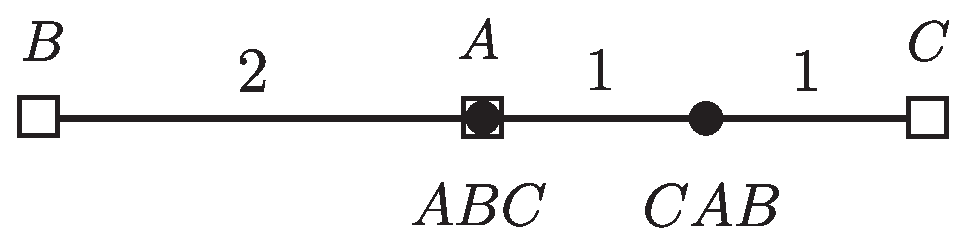
\includegraphics[scale=0.3]{awn.eps}
\caption{\label{fig:1} Tight example for the Adapted Weighted Uncovered rule. Candidates and voters are denoted by squares and circles, respectively. }
\end{center}
\end{figure}

\end{example}

\section{Improving the Distortion}\label{sec:im}

The tools of Lemma \ref{lem:31} and \ref{lem:32} allow us to design more involved mechanisms. In this section, we propose a mechanism which selects a candidate from a subset of candidates, if this set is not empty. In particular, when the number of candidates is at most 6, the mechanism can always successfully return a candidate, and the distortion is at most $2\sqrt2+1\approx 3.828$, improving the distortion 4.236 of Adapted Weighted Uncovered.

\vspace{2mm}\hspace{-3.5mm}\textbf{Mechanism 2.}  {\sc($Cov_{su}(y)$ rule.)} Let $y\ge 1$ be a constant. The $Cov_{su}(y)$-set is the set of candidates $A\in \mathcal C$ such that for any candidate $B\neq A$, we have
 \begin{enumerate}
\item either $|BA|\ge \frac{2}{y+1}$,
\item or there exists an intermediary candidate $C\ne A,B$ such that $|BA|+\frac{y-1}{2}|CA|\ge 1$ and $|BC|\ge \frac{2}{y+1}$.
 \end{enumerate}
The rule selects an arbitrary candidate in the $Cov_{su}(y)$-set if possible.


\begin{theorem}\label{thm:dis}
 If the $Cov_{su}(y)$-set is non-empty, then $Cov_{su}(y)$ rule has distortion of at most $y$.
 \end{theorem}
\begin{proof}
 Let $A\in \mathcal C$ be a candidate in the $Cov_{su}(y)$-set. Consider an arbitrary candidate $B\neq A$. If $|BA|\ge \frac{2}{y+1}$, by Lemma \ref{lem:31}, we have
$$\frac{S(B,d)}{S(A,d)}\le \frac{2}{|BA|}-1\le \frac{2}{\frac{2}{y+1}} - 1=y.$$
  If $|BC|\ge \frac{2}{y+1}$ and $|BA|+\frac{y-1}{2}|CA|\ge 1$, by Lemma \ref{lem:32}, we also have
  \begin{align*}
 \frac{S(B,d)}{S(A,d)}\le &\ max\{\frac{2}{|BC|}-1 , \frac{2(1-|BA|)}{|CA|} + 1\} \\
 \le& \ max\{\frac{2}{\frac{2}{y+1}}-1 , \frac{2(1-|BA|)}{\frac{2}{y-1}(1-|BA|)} + 1\} = y.
 \end{align*}
 \end{proof}

An immediate question is, when the $Cov_{su}(y)$-set is non-empty? Before that, we give some necessary definitions.

 \begin{definition}
 \begin{enumerate}
 \item For two candidates $A$ and $B$, we say $A\times B$, if $|BA|<\frac{2}{y+1}$ and for any $C\neq A,B$, either $|BA|+\frac{y-1}{2}|CA|<1$ or $|BC|<\frac{2}{y+1}$.
\item A \emph{$y$-covered-cycle} in the weighted tournament graph is a vertex  sequence $(A_1,A_2,\ldots,A_k,A_{k+1}=A_1)$, such that $A_i\times A_{i+1}$ for any $i=1,2,\ldots,k$, in which all vertices are distinct except for $A_1$ and $A_{k+1}$.
    \end{enumerate}
    \end{definition}
     Note that $A\times B$ implies candidate $B$ does not satisfy the conditions in Mechanism 2, and thus $Cov_{su}(y)$ rule selects a candidate $A$ such that for any other candidate $B$, $A\times B$ does not hold. The length of such a $y$-covered-cycle is the number of distinct vertices.  Let $L$ be the length of the longest $y$-covered-cycle in the weighted tournament graph.

 \begin{lemma}\label{lem:n3}
 When $n=3$, the $Cov_{su}(3)$-set is non-empty, and the distortion of $Cov_{su}(3)$ rule is at most $3$.
 \end{lemma}

 \begin{proof}
 Assume for contradiction that the $Cov_{su}(3)$-set is empty. Let $A,B,C$ be the three candidates in this election. W.l.o.g. we can assume $A\times B,B\times C,C\times A$, indicating $|BA|,|CB|,|AC|<0.5$. Then we have $|AB|,|BC|,|CA|\ge 0.5$. Hence, by the definition, there must be $|BA|+|CA|<1,|CB|+|AB|<1$ and $|AC|+|BC|<1$. Summing up these three inequalities, it derives $3<3$, a contradiction.
 \end{proof}

 Before analyzing the case with more candidates, we give a necessary condition for the edge weights in the weighted tournament graph.

 \begin{lemma}\label{lem:loop}
 For any $t$ ($t\ge 3$) candidates $A_1,...,A_t$, we have
$$ \sum_{i = 1}^{t-1}{|A_iA_{i+1}|}+|A_tA_1| \ge 1. $$
\end{lemma}

\begin{proof}
 We use induction to prove this claim. First consider three candidates $A,B,C$, and we have
 \begin{align*}
 & |AB|+|BC|+|CA| \\
 = &\ (|ABC|+|ACB|+|CAB|) + (|ABC|+|BAC|+|BCA|)\\
 + &\ (|CAB|+|CBA|+|BCA|) \\
 = &\ (|ABC|+|ACB|+|CAB|+|BAC|+|BCA|+|CBA|) \\
 + &\ (|ABC|+|BCA|+|CAB|) \\
 = &\ 1 + (|ABC|+|BCA|+|CAB|)
 \ge 1.
\end{align*}

Suppose the claim is true when $t=k$. Now consider $t=k+1$, and we have
 \begin{align*}
  \sum_{i = 1}^{k}&{|A_iA_{i+1}|}+|A_{k+1}A_1|\\
 =  \sum_{i = 1}^{k-1}&(|A_iA_{i+1}| + |A_{k}A_1|)+ \\
&(|A_{k+1}A_{1}| + |A_{1}A_{k}| +|A_kA_{k+1}|) - 1 \\
 \ge \ 1 + &1 - 1 = 1,
\end{align*}
which completes the proof.
\end{proof}

%Lemma \ref{lem:loop} also indicates that $|A_1A_m| \le \sum_{i = 1}^{m-1}{|A_iA_{i+1}|}.$
In the remainder of this section, we only consider $y=2\sqrt2+1 \approx 3.828$, and  denote $\lambda=\frac{2}{y+1}=\sqrt2-1$. Using the above lemma, we prove the distortion for the cases $n=4,5,6$ in the following.

\begin{lemma}\label{lem:n4}
 There is no $y$-covered-cycle of length 3 or 4. In addition, when $n=4$, the $Cov_{su}(2\sqrt2+1)$-set is non-empty.
 \end{lemma}
\begin{proof}
Suppose there is a $y$-covered-cycle $(A,B,C,A)$  of length 3.  We have $|AB|,|BC|,|CA|>1-\lambda=2-\sqrt2$ and $|BA|+\sqrt2|CA|, |CB|+\sqrt2|AB|, |AC|+\sqrt2|BC|<1$. Summing up the last three inequalities, it derives $(|BA|+|CB|+|AC|)+\sqrt2\cdot (|CA|+|BC|+|AC|)<3$. However, by Lemma \ref{lem:loop}, we have
\begin{align*}
&\ (|BA|+|CB|+|AC|)+\sqrt2\cdot (|CA|+|BC|+|AC|)\\
\ge &\ 1+\sqrt2\cdot (|CA|+|BC|+|AC|)\\
\ge &\ 1+3\sqrt2(2-\sqrt2) > 3,
\end{align*}
a contradiction.

Suppose there is a $y$-covered-cycle $(A,B,C,D,A)$  of length 4. Define an edge set $T:=\{(B,A),\\(C,B),(D,C),(A,D)\}$
in the weighted tournament graph. Clearly all edges in $T$ have weights less than $\lambda$. Let $k$ be the number of edges in $E\backslash T$, whose weights are less than $\lambda$. There are 3 cases.

 \vspace{1mm}\noindent\textbf{Case 1: $k=0$.}  Then we have $|BA|+\sqrt2|DA|, |CB|+\sqrt2|AB|, |DC|+\sqrt2|BC|, |AD|+\sqrt2|CD|<1$. Summing up these 4 inequalities, it derives $(|BA|+|CB|+|DC|+|AD|)+\sqrt2\cdot (|DA|+|CD|+|BC|+|AB|)<4$. However, by Lemma \ref{lem:loop}, the left hand side is at least $1+4\sqrt2\cdot (2-\sqrt2)>4$, a contradiction.

 \vspace{1mm}\noindent\textbf{Case 2: $k=1$.} W.l.o.g. assume $|CA|<\sqrt2-1$. We have $|DC|+\sqrt2|BC|,|AD|+\sqrt2|CD|<1$, which immediately gives
 $\sqrt2\cdot (|DC|+\sqrt2|BC|)+(|AD|+\sqrt2|CD|)<\sqrt2+1$.
  But the left hand side of this inequality is larger than $2|BC|+\sqrt2>2*0.5+\sqrt2=\sqrt2+1$, a contradiction.

 \vspace{1mm}\noindent\textbf{Case 3: $k=2$.} The analysis is similar to that in Case 2.

Therefore, there is no $y$-covered-cycle of length 3 or 4.  When $n=4$, an empty $Cov_{su}(2\sqrt2+1)$-set indicates the existence of a $y$-covered-cycle of length 3 or 4, since $A\times B$ and $B\times A$ cannot hold simultaneously. Thus the $Cov_{su}(2\sqrt2+1)$-set is non-empty when $n=4$.
\end{proof}


  We say $A\rightarrow B$ if $|BA|< \lambda$, and $A\nrightarrow B$ if $|BA|\ge \lambda$.  In the weighted tournament graph, a \emph{$\lambda$-path} is a vertex sequence $(A_1,A_2,\ldots,A_k)$, such that $A_i\rightarrow A_{i+1}$ for $i=1,2,\ldots,k-1$, in which all vertices are distinct.  Further, a \emph{$\lambda$-cycle} is a vertex sequence $(A_1,A_2,\ldots,A_k,A_{k+1}=A_1)$, such that $A_i\rightarrow A_{i+1}$ for any $i=1,2,\ldots,k$,  in which the only repeated vertices are the first and last vertices. Clearly, $A\times B$ implies $A\rightarrow B$, and any $y$-covered-cycle must be a $\lambda$-cycle.


\begin{lemma}\label{lem:n5}
There is no $y$-covered-cycle of length 5.  In addition, when $n=5$, the $Cov_{su}(2\sqrt2+1)$-set is non-empty.
 \end{lemma}

\begin{proof}
 %First we can easily get that, if we select an arbitrary vertex $A$ from the 3-vertices $\lambda$-cycle $(A,B,C,A)$, then $|BA|+\sqrt2\cdot |CA|\ge 1$ and $|BC|>\lambda$. Therefore we have $\frac{S(B,d)}{S(A,d)}\le y \approx 3.828$.

%Then consider a $\lambda$-path $(A,B,C,D)$. We can also get that $|CB|+\sqrt2\cdot |AB|<1$ and $|DC|+\sqrt2\cdot |BC|<1$ cannot hold at the same time. Therefore, if there is neither $A\rightarrow C$ nor $B\rightarrow D$, then we have $min\{\frac{S(C,d)}{S(B,d)}, \frac{S(D,d)}{S(C,d)}\}\le 2\sqrt2+1$.

%Back to the 5-vertices $y$-covered-cycle set, we call $\{A\rightarrow C,B\rightarrow D,C\rightarrow E,D\rightarrow A,E\rightarrow B\}$ an edge set $T$. Let $k$ be the number of edges of $T$ that appears in the graph, thus there are 6 cases. And we can prove by analyzing all the cases.
We first prove two useful claims.

 \smallskip\noindent\textbf{Claim 1.} For any length-3 $\lambda$-cycle $(A,B,C,A)$, $A\times B$ does not hold. %we have $\frac{S(B,d)}{S(A,d)}\le y$.

 For such a $\lambda$-cycle, we have $|BA|+\sqrt2\cdot |CA|\ge (1-|AC|-|CB|) + \sqrt2\cdot (2-\sqrt2) \ge (3-2\sqrt2) + (2\sqrt2-2) \ge 1$ and $|BC|\ge 1-\lambda >\lambda$. Thus, $A\times B$ does not hold. %It derives $\frac{S(B,d)}{S(A,d)}\le y$, using the proof of Theorem \ref{thm:dis}.

%Then consider any $\lambda$-path $(A,B,C,D)$. If $|CB|+\sqrt2 \cdot |AB|<1$, then $|BA|-|CB|>(\sqrt2-1)\cdot(1-|BA|)=(\sqrt2-1)\cdot|AB|>(\sqrt2-1)\cdot(2-\sqrt2)=3\sqrt2-4$. So if we want both $|CB|+\sqrt2 \cdot |AB|<1$ and $|DC|+\sqrt2 \cdot |BC|<1$ hold, it will contradict with the definition of $\lambda$-path, because $|BA|>|CB|+3\sqrt2-4>|DC|+6\sqrt2-8>6\sqrt2-8>\lambda$. Thus if there is neither $A\rightarrow C$ nor $B\rightarrow D$, then we have $min\{\frac{S(C,d)}{S(B,d)}, \frac{S(D,d)}{S(C,d)}\}\le y$.

\smallskip\noindent\textbf{Claim 2.} For any $\lambda$-path $(A,B,C,D)$, if $A\nrightarrow C$ and $B\nrightarrow D$, then $B\times C$ and $C\times D$ cannot hold at the same time.

 Note that $\sqrt2(|CB|+\sqrt2|AB|)+(|DC|+\sqrt2|BC|)=\sqrt2+2|AB|+|DC|\ge \sqrt2 + 2(1-\lambda)+0>\sqrt2+1$. Then, for $\lambda$-path $(A,B,C,D)$, it must have either $|CB|+\sqrt2 \cdot |AB|\ge1$ or $|DC|+\sqrt2 \cdot |BC|\ge1$, implying this claim.

\medskip Now we assume for contradiction that there is a $y$-covered-cycle $\Gamma=(A,B,C,D,E,A)$ of length 5, and define edge set $T=\{(A,C),(B,D),(C,E),(D,A),(E,B)\}$, as shown in Figure \ref{fig:3}. Let $k$ be the number of edges of $T$ whose weight is larger than $1-\lambda$. In the following we discuss 4 cases w.r.t. the value of $k$.

\begin{figure}[htpb]
\begin{center}

\includegraphics[scale=0.18]{n5.eps}
\caption{\label{fig:3} A $y$-covered-cycle $\Gamma=(A,B,C,D,E,A)$. Edge set $T$ consists of dashed edges. }
\end{center}
\end{figure}


\noindent\textbf{Case 1: $k=0$.} We have $A\nrightarrow C$ and $B\nrightarrow D$. By Claim 2, $B\times C$ and $C\times D$ cannot hold at the same time, a contradiction with the assumption of  $y$-covered-cycle $\Gamma$.
%Based on Claim 2, we consider an arbitrary $\lambda$-path such as $(A,B,C,D)$. \bluecomment{Since $|AB|,|BC|>1-\lambda$, it is easy to see that there must be either $|CB|+\sqrt2 \cdot |AB|\ge 1$ or $|DC|+\sqrt2 \cdot |BC|\ge 1$.  If $|CB|+\sqrt2 \cdot |AB|\ge 1$, combined with $|CA|\ge \lambda$, it leads to a contradiction with $B\times C$. If $|DC|+\sqrt2 \cdot |BC|\ge 1$, combined with $|DB|\ge \lambda$, it leads to a contradiction with $C\times D$.}

\noindent\textbf{Case 2: $k=1$.} W.l.o.g. assume $A\rightarrow C$. We have $B\nrightarrow D$ and $C\nrightarrow E$. By Claim 2, $C\times D$ and $D\times E$ cannot hold at the same time, a contradiction with the assumption of  $y$-covered-cycle $\Gamma$.
%Considering the $\lambda$-path $(B,C,D,E)$, it is easy to see that either $|CB|+\sqrt2 \cdot |AB|\ge 1$ or $|DC|+\sqrt2 \cdot |BC|\ge 1$, according to case 1, we can prove with the similar process.

\noindent\textbf{Case 3: $k=2$.} There are two different subcases. The first one is typically represented by $A\rightarrow C, B\rightarrow D$. Then we have $C\nrightarrow E$ and $D\nrightarrow A$, which derives a contradiction in $\lambda$-path $(C,D,E,A)$ by Claim 2. The second one is typically represented by $A\rightarrow C\rightarrow E$. Then we have $D\nrightarrow A$ and $E\nrightarrow B$, which derives a contradiction in $\lambda$-path $(D,E,A,B)$ by Claim 2.
%Considering the cyclic symmetry, there are 2 different situations. The former one is $A\rightarrow C, B\rightarrow D$ and we only need to observe the path $(C,D,E,A)$ in the same way as case 1. The latter one is $A\rightarrow C\rightarrow E$ and we only need observe the path $(D,E,A,B)$, also a contradiction.

\noindent\textbf{Case 4: $k\ge 3$.} There must be a length-2 $\lambda$-path using edges in $T$, without loss of generality assumed to be  $A\rightarrow C\rightarrow E$. Then there is a $\lambda$-cycle $(E,A,C,E)$. However, by Claim 1, $E\times A$ does not hold, a contradiction with $\Gamma$.

%There are three different subcases. If $B\rightarrow D$, Then we have $D\nrightarrow A$ and $E\nrightarrow B$, which derives a contradiction in $\lambda$-path $(D,E,A,B)$ by Claim 2. If $D\rightarrow A$, then there is a $\lambda$-cycle $(C,D,A,C)$. However, by Claim 1, $C\times D$ does not hold, a contradiction with $\Gamma$. If $E\rightarrow B$ and at this time we can select $E$ as the winner for the cycle $(E,A,C,E)$ and $(E,B,C,E)$, a contradiction.


%\noindent\textbf{Case 5: $k=4$.} W.l.o.g. assume there is not $E\rightarrow B$ and we can select $C$ as the winner for the cycle $(C,D,A,C)$ and $(C,E,A,C)$, a contradiction.

%\noindent\textbf{Case 6: $k=5$.} This time we can select any candidate as the winner and we can all find the cycle same as above, with a contradiction.

When $n=5$, if the $Cov_{su}(2\sqrt2+1)$-set is empty, then there must be a $y$-covered-cycle of length at most 5. However, such a $y$-covered-cycle does not exist by the above discussions. So the $Cov_{su}(2\sqrt2+1)$-set is non-empty.

\end{proof}


\begin{lemma}\label{lem:n6}
There is no $y$-covered-cycle of length 6.  In addition, when $n=6$, the $Cov_{su}(2\sqrt2+1)$-set is non-empty.
\end{lemma}

\begin{proof}
 Now we assume for contradiction that there is a $y$-covered-cycle $(A,B,C,D,E,F,A)$ of length 6. Define edge set $T=\{(A,C),(B,D),(C,E),(D,F),(E,A),(F,B)\}$. Let $k$ also be the number of edges of $T$ whose weight is larger than $1-\lambda$. In the same way as length 5, we divide it into 7 cases. But according to the proof of last lemma, it's easy to know that when $k=0,1$, the proof is completely the same, and that when $n=2$, the proof is nearly the same except an additional similar situation, thus omitted, leaving other 4 cases i.e., for $k=3,4,5,6$.

\noindent\textbf{Case 1: $k=3$.} Because there should not be 4-vertices $\lambda$-path according to the last lemma (or it will be a contradiction), the three edges can only be $A\rightarrow C\rightarrow E\rightarrow A$. If $A\rightarrow D$, then there will be a length-3 $\lambda$-cycle $(A,D,E,A)$, causing a contradiction with $D\times E$. So by symmetry, we have $A\nrightarrow D,C\nrightarrow F,E\nrightarrow B$. Also, $B\nrightarrow F,F\nrightarrow D,D\nrightarrow B$, or it will also lead to a length-3 $\lambda$-cycle.

We have $|DB|,|FD|,|BD|\ge \sqrt2-1$, and $|BA|+\sqrt2\cdot |FA|, |DC|+\sqrt2\cdot |BC|, |FE|+\sqrt2\cdot |DE|<1$, or it will be contradict with the $y$-covered cycle. So $|FA|,|BC|,|DE|<\frac{\sqrt2}{2}$, i.e., $|AF|,|CB|,|ED|>1-\frac{\sqrt2}{2}$. Besides, we have $|CB|+\sqrt2|DB|,|CB|+\sqrt2|FB|,|ED|+\sqrt2|FD|,|ED|+\sqrt2|BD|,|AF|+\sqrt2|BF|,|AF|+\sqrt2|DF|<1$. Add these 6 inequalities together, and we get $2\cdot (|CB|+|ED|+|AF|)+3\cdot \sqrt2 < 6$. Also because $2\cdot(|CB|+|ED|+|AF|)>6-3\cdot \sqrt2$, we get $6<6$, with contradiction.

\noindent\textbf{Case 2: $k=4$.}
Considering cyclic symmetry, we should consider 2 situations and others can be proved to a contradiction with the same method as 3-vertices cycle and 4-vertices path.

First focus on $A\rightarrow C\rightarrow E\rightarrow A$ and $D\rightarrow F$.
This is easier than 3 elements. We should have $|BA|+\sqrt2\cdot |FA|<1$ and $|AF|+\sqrt2|DF|<1$. So add these two to get $2>|BA|+\sqrt2\cdot|FA|+|AF|+\sqrt2\cdot|DF|>1+|BA|+(\sqrt2-1)\cdot|FA|+\sqrt2\cdot |DF|
> 1 + 0 + (2\sqrt2-1)(2-\sqrt2)=5\sqrt2-5>2$, with contradiction.

Second focus on $A\rightarrow C\rightarrow E$ and $D\rightarrow F\rightarrow B$.
Similar to last situation, it is easy to know $|FE|+\sqrt2|CE|<1, |AF|+\sqrt2|EF|<1$. So add these together to get $2>|FE|+\sqrt2\cdot|CE|+|AF|+\sqrt2\cdot|EF|>1+|AF|+(\sqrt2-1)\cdot|EF|+\sqrt2\cdot |CE|p> 1 + 0 + (2\sqrt2-1)(2-\sqrt2)=5\sqrt2-5>2$, with contradiction.

\noindent\textbf{Case 3: $k=5$.} W.l.o.g we assume $E\rightarrow A$ is not in the graph. We can get contradiction with the same proof as the second situation in case 2.

\noindent\textbf{Case 4: $k=6$.} If $A\rightarrow D$, then we can get length-3 $\lambda$-cycle $(A,D,E,A)$, leading to a contradiction. Therefore, we have $A\nrightarrow D,D\nrightarrow A,B\nrightarrow E,E\nrightarrow B,C\nrightarrow F,F\nrightarrow C$. Also we have
$|BA|+\sqrt2|FA|,|CB|+\sqrt2|AB|,|DC|+\sqrt2|BC|,|ED|+\sqrt2|CD|,|FE|+\sqrt2|DE|,|AF|+\sqrt2|EF|<1$.

Add them together, and we can get
$ 6 > (|BA|+|CB|+|DC|+|ED|+|FE|+|AF|) + \sqrt2\cdot (6-|CA|-|DB|-|EC|-|FD|-|AE|-|BF|) $.
Because according to Lemma \ref{lem:loop}, $|CA|<|BA|+|CB|$, we have
$6>6\sqrt2-(\sqrt2-0.5)\cdot (|CA|+|DB|+|EC|+|FD|+|AE|+|BF|)>6\sqrt2-6(\sqrt2-0.5)\cdot(\sqrt2-1)=15\cdot (\sqrt2-1)>6$, with contradiction.

When $n=6$, if the $Cov_{su}(2\sqrt2+1)$-set is empty, then there must be a $y$-covered-cycle of length 3 or 4 or 5 or 6, since  $A\times B$ and $B\times A$ cannot hold simultaneously. So the $Cov_{su}(2\sqrt2+1)$-set is nonempty.
\end{proof}

% Assume the set is empty and $A\times B\times C\times D\times E\times F\times A$, and let set $T$ be $\{A\rightarrow C,B\rightarrow D,C\rightarrow E,D\rightarrow F,E\rightarrow A,F\rightarrow B\}$.
%In the same way, Let $k$ denote the number of edges in $T$ that appear in the graph. According to the last lemma, it's easy to know that when $k=0,1,2$, the proof is the same, thus omitted, leaving other 4 cases.
%
%\noindent\textbf{Case 1: $k=3$.} Because there should not be 4-vertices path similar to the last lemma (or it will be a contradiction), the three edges can only be $A\rightarrow C\rightarrow E\rightarrow A$. If $A\rightarrow D$, then we can select $D$. So there should not be $A\rightarrow D,C\rightarrow F,E\rightarrow B$. Also, there should not be $B\rightarrow F,F\rightarrow D,D\rightarrow B$.
%
%We have $|DB|,|FD|,|BD|\ge \sqrt2-1$, and $|BA|+\sqrt2\cdot |FA|, |DC|+\sqrt2\cdot |BC|, |FE|+\sqrt2\cdot |DE|<1$, or it will be contradict with the $y$-covered cycle. So $|FA|,|BC|,|DE|<\frac{\sqrt2}{2}$, i.e., $|AF|,|CB|,|ED|>1-\frac{\sqrt2}{2}$. Besides, we have p $|CB|+\sqrt2|DB|,|CB|+\sqrt2|FB|,|ED|+\sqrt2|FD|,|ED|+\sqrt2|BD|,|AF|+\sqrt2|BF|,|AF|+\sqrt2|DF|<1$. Add these 6 inequalities together, and we get $2\cdot (|CB|+|ED|+|AF|)+3\cdot \sqrt2 < 6$. Also because $2\cdot(|CB|+|ED|+|AF|)>6-3\cdot \sqrt2$, we get $6<6$, with contradiction.
%
%\noindent\textbf{Case 2: $k=4$.}
%Considering cyclic symmetry, we should consider 2 situations and others can be proved to a contradiction with the same method as 3-vertices cycle and 4-vertices path.
%
%First focus on $A\rightarrow C\rightarrow E\rightarrow A$ and $D\rightarrow F$.
%This is easier than 3 elements. We should have $|BA|+\sqrt2\cdot |FA|<1$ and $|AF|+\sqrt2|DF|<1$. So add these two to get $2>|BA|+\sqrt2\cdot|FA|+|AF|+\sqrt2\cdot|DF|>1+|BA|+(\sqrt2-1)\cdot|FA|+\sqrt2\cdot |DF|
%> 1 + 0 + (2\sqrt2-1)(2-\sqrt2)=5\sqrt2-5>2$, with contradiction.
%
%Second focus on $A\rightarrow C\rightarrow E$ and $D\rightarrow F\rightarrow B$.
%Similar to last situation, it is easy to know $|FE|+\sqrt2|CE|<1, |AF|+\sqrt2|EF|<1$. So add these together to get $2>|FE|+\sqrt2\cdot|CE|+|AF|+\sqrt2\cdot|EF|>1+|AF|+(\sqrt2-1)\cdot|EF|+\sqrt2\cdot |CE|p> 1 + 0 + (2\sqrt2-1)(2-\sqrt2)=5\sqrt2-5>2$, with contradiction.
%
%\noindent\textbf{Case 3: $k=5$.} W.l.o.g we assume $E\rightarrow A$ is not in the graph. We can get contradiction with the same proof as the second situation in case 2.
%
%\noindent\textbf{Case 4: $k=6$.} If $A\rightarrow D$, then $D$ can be selected. Therefore, none of $A\rightarrow D,D\rightarrow A,B\rightarrow E,E\rightarrow B,C F,F C$ appears. We have
%$|BA|+\sqrt2|FA|,|CB|+\sqrt2|AB|,|DC|+\sqrt2|BC|,|ED|+\sqrt2|CD|,|FE|+\sqrt2|DE|,|AF|+\sqrt2|EF|<1$.
%
%Add them together, and we can get
%$ 6 > (|BA|+|CB|+|DC|+|ED|+|FE|+|AF|) + \sqrt2\cdot (6-|CA|-|DB|-|EC|-|FD|-|AE|-|BF|) $.
%Because according to Lemma \ref{lem:loop}, $|CA|<|BA|+|CB|$, we have
%$6>6\sqrt2-(\sqrt2-0.5)\cdot (|CA|+|DB|+|EC|+|FD|+|AE|+|BF|)>6\sqrt2-6(\sqrt2-0.5)\cdot(\sqrt2-1)=15\cdot (\sqrt2-1)>6$, with contradiction.
%
%When $n=6$, if the $A5(2\sqrt2+1)$-set is empty, then there must be a $y$-covered-cycle of length 3 or 4 or 5 or 6, since  $A\times B$ and $B\times A$ cannot hold simultaneously. So the $A5(2\sqrt2+1)$-set is nonempty.
%
%If there are 3 elements, then it can only be $A\rightarrow_{0.414'}C\rightarrow_{0.414'}E\rightarrow_{0.414'}A$, or it will appear the path proposed last paragraph.
%If $A\rightarrow_{0.414'}D$, then we can select $D$. So there should not be $A\rightarrow_{0.414'}D,C\rightarrow_{0.414'}F,E\rightarrow_{0.414'}B$. Also, there should not be $B\rightarrow_{0.414'}F,F\rightarrow_{0.414'}D,D\rightarrow_{0.414'}B$.
%
%Because $|BD|',|DF|',|FB|'>\sqrt2-1$, we have $|AB|'+\sqrt2\cdot |AF|', |CD|'+\sqrt2\cdot |CB|', |EF|'+\sqrt2\cdot |ED|'<1$. So $|AF|',|CB|',|ED|'<\frac{\sqrt2}{2}$, i.e., $|FA|,|BC|,|DE|>1-\frac{\sqrt2}{2}$. Besides, we have $|BC|'+\sqrt2|BD|',|BC|'+\sqrt2|BF|',|DE|'+\sqrt2|DF|',|DE|'+\sqrt2|DB|',|FA|'+\sqrt2|FB|',|FA|'+\sqrt2|FD|'<1$.
%
%Add these 6 inequalities together, we get $2\cdot (|BC|'+|DE|'+|FA|')+3\cdot \sqrt2 < 6$. Also because $2\cdot(|BC|'+|DE|'+|FA|')>6-3\cdot \sqrt2$, we get $6<6$, with contradiction.
%
%If there are 4 elements, we should consider 2 situations.
%
%First focus on $A\rightarrow_{0.414'}C\rightarrow_{0.414'}E\rightarrow_{0.414'}A$ and $D\rightarrow_{0.414'}F$.
%The method is easier than 3 elements. We should have $|AB|'+\sqrt2\cdot |AF|'<1$. Besides, $|FA|'+\sqrt2|FD|'<1$, so we add these two to get $2>|AB|'+\sqrt2\cdot|AF|'+|FA|'+\sqrt2\cdot|FD|'>1+|AB|'+(\sqrt2-1)\cdot|AF|'+\sqrt2\cdot |FD|'
%> 1 + 0 + (2\sqrt2-1)(2-\sqrt2)=5\sqrt2-5>2$, with contradiction.
%
%Second focus on $A\rightarrow_{0.414'}C\rightarrow_{0.414'}E$ and $D\rightarrow_{0.414}F\rightarrow_{0.414'}B$.
%Similar to last situation, it is easy to know $|EF|'+\sqrt2|EC|'<1, |FA|'+\sqrt2|FE|'<1$. So add these together to get $2>|EF|'+\sqrt2\cdot|EC|'+|FA|'+\sqrt2\cdot|FE|'>1+|FA|'+(\sqrt2-1)\cdot|FE|'+\sqrt2\cdot |EC|'> 1 + 0 + (2\sqrt2-1)(2-\sqrt2)=5\sqrt2-5>2$, with contradiction.
%
%If there are 5 elements, we assume $E\rightarrow_{0.414'}A$ is not in the graph. We can get contradiction with the same proof as the second situation in 4 elements.
%
%If there are 6 elements, all the edges int the set appear. If $A\rightarrow_{0.414'}D$, then $D$ can be selected. Therefore, none of $A\rightarrow_{0.414'}D,D\rightarrow_{0.414'}A,B\rightarrow_{0.414'}E,E\rightarrow_{0.414'}B,C\rightarrow_{0.414'}F,F\rightarrow_{0.414'}C$ appears. We have
%$|AB|'+\sqrt2|AF|',|BC|'+\sqrt2|BA|',|CD|'+\sqrt2|CB|',|DE|'+\sqrt2|DC|',|EF|'+\sqrt2|ED|',|FA|'+\sqrt2|FE|'<1$.
%
%Add them together, and we can get
%$ 6 > (|AB|'+|BC|'+|CD|'+|DE|'+|EF|'+|FA|') + \sqrt2\cdot (6-|AC|'-|BD|'-|CE|'-|DF|'-|EA|'-|FB|') $.
%Because according to Lemma 3.3, $|AC|'<|AB|'+|BC|'$, we have
%$6>6\sqrt2-(\sqrt2-0.5)\cdot (|AC|'+|BD|'+|CE|'+|DF|'+|EA|'+|FB|')>6\sqrt2-6(\sqrt2-0.5)\cdot(\sqrt2-1)=15\cdot (\sqrt2-1)>6$, with contradiction.


 %If $distortion>2\sqrt2+1$, then the number of vertices of a $y$-covered-cycle consisting of $A\times B...\times A$ must be $>6$. And we also guess for some $n>6$, 3.828-A1 set is not empty. Therefore we can get a stronger conclusion.
 \begin{theorem}
 If all $\lambda$-cycles in the weighted tournament graph have length at most 6, then the $Cov_{su}(2\sqrt2+1)$-set is non-empty, and $Cov_{su}(2\sqrt2+1)$ rule has distortion at most $2\sqrt2+1\approx 3.828$ for the social utility objective.
\end{theorem}

\begin{proof}
Note that any $y$-covered-cycle must be a $\lambda$-cycle, indicating that the length of any $y$-covered-cycle is at most 6. However, by Lemma \ref{lem:n4}, \ref{lem:n5} and \ref{lem:n6}, there is no $y$-covered-cycle of length 3,4,5 or 6. Therefore, there exists no $y$-covered-cycle in the weighted tournament graph. We can easily find a candidate $A$ such that for any $B\neq A$, $A\times B$ does not hold. Then $A$ is in the $Cov_{su}(y)$-set. By Theorem \ref{thm:dis}, the distortion is at most $2\sqrt2+1$.
 \end{proof}

We believe that the $Cov_{su}(2\sqrt2+1)$-set is non-empty for more general situations when there is some $\lambda$-cycle of length larger than 6. We are not able to provide a proof or a counterexample to show whether there is $y$-covered-cycle of length at least 7, since there are more and more cases to discuss and it is hard to generalize. We leave this as an open question.

The following example shows the tightness of the distortion $2\sqrt2+1$ for $Cov_{su}(2\sqrt2+1)$ rule.
\begin{figure}[htpb]
\begin{center}
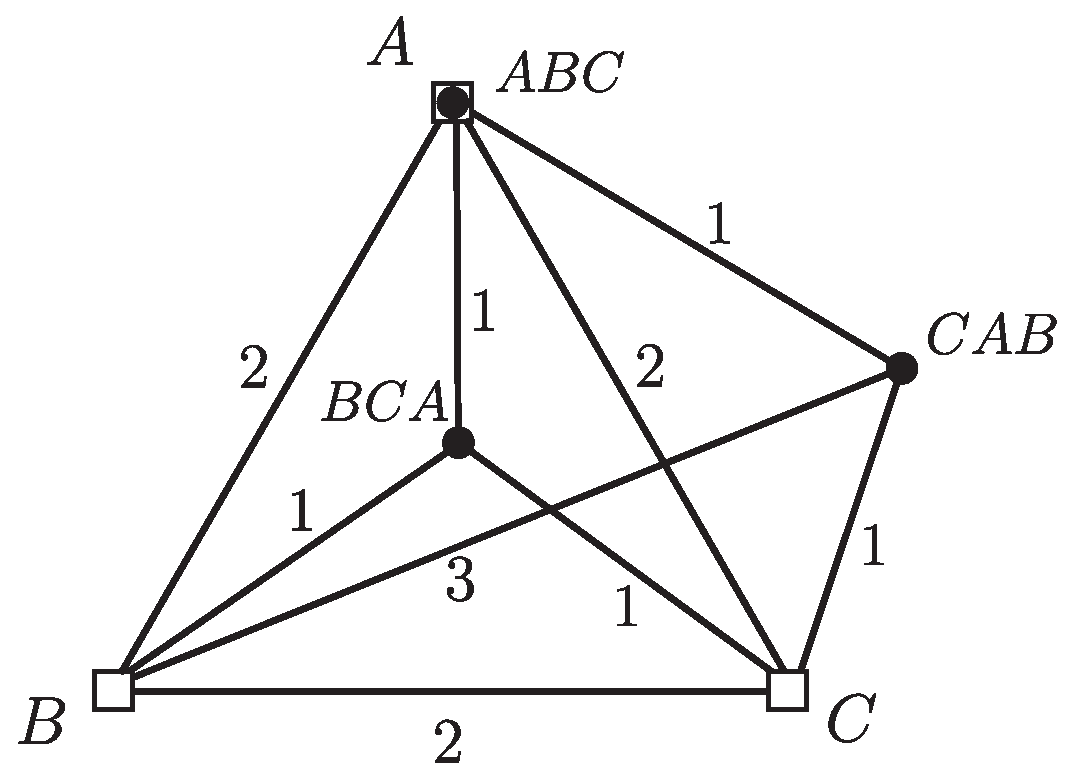
\includegraphics[scale=0.3]{a5.eps}
\caption{\label{fig:2} Tight example for $Cov_{su}(2\sqrt2+1)$ rule.}
\end{center}
\end{figure}

\begin{example}
Let $\mathcal C=\{A,B,C\}$. Each voter belongs to one set of $BCA,ABC,CAB$, and define $|BCA|=3-2\sqrt2,|ABC|=|CAB|=\sqrt2-1$. It is easy to see that candidate $A$ is in the $Cov_{su}(2\sqrt2+1)$ set, and can be selected by $Cov_{su}(2\sqrt2+1)$ rule. However, the underlying metric space may be as shown in Figure \ref{fig:2}.
At this time, we have $S(A,d)=2-\sqrt2$ and $S(B,d)=3\sqrt2-2$, indicating a distortion at least $\frac{S(B,d)}{S(A,d)}=2\sqrt2+1$.

This example can be easily extended to that with more than three candidates, by setting extra candidates very far away.
\end{example}

%\begin{example}
%Let $A,B,C$ be candidates and $P=ABC,Q=BCA,R=CAB$. Consider this situation: $|Q|=3-2\sqrt2,|P|=|R|=\sqrt2-1$. In metric space, there are $d(B,A)=d(A,C)$, $ d(B,P)=d(C,P)=d(B,A),d(A,P)=0, d(B,Q)=d(A,Q)=d(C,Q)=0.5d(B,A), d(A,R)=d(C,R)=0.5d(A,C), d(B,R)=d(A,B)+d(A,R)=1.5d(A,C)$. At this time, it's obvious that $\frac{S(A,d)}{S(B,d)}=2\sqrt2+1$ and $A,B$ are both in the $A5(2\sqrt2+1)$ set.
%\end{example}

%We believe that there is at least one candidate in a 3.828-A5 set at least for some not very large $n$ and $L$, and leave this as an open question.




\section{Extension: Minimizing Social Cost}\label{sec:min}

In this section, we extend the results in Section \ref{sec:im} to the problem of minimizing social cost. The cost of each voter is the distance to the winner selected by the rule, and the social cost is the total cost of all voters. Under the social cost objective, the lower bound on distortion of voting rules is 3 \cite{anshelevich2015approximating}, and the best known distortion is $2+\sqrt5\approx 4.236$, achieved by the Weighted Uncovered rule \cite{munagala2019improved}.

Some special cases have improved distortion. Anshelevich \emph{et al.} \cite{anshelevich2015approximating}  proved that the Ranked Pairs rule achieves the best possible distortion bound 3 when the tournament graph  has  maximum cycle size no more than 4. It indicates that this rule is optimal when $n=3$ or 4. However, its distortion is at least 5 in general. We note that when $n=3$, Ranked Pairs is equivalent to the following rule: select the candidate with maximum min-weight, where the min-weight of a candidate is defined as the minimum weight of all its outgoing edges in the weighted tournament graph. %This simplifies the process of selection by reducing the time.

Now we apply a dual idea of Mechanism 2 to the social cost objective, and provide improved distortion for some special cases. In particular, we show that there is a mechanism with distortion at most 3.828 when $n=5$ or $n=6$, improving the best known distortion 4.236 before.


\iffalse
\begin{theorem}\label{thm:A2}
 When $n=3$, the $distortion$ of $A2\ rule$ is at most 3.
 \end{theorem}

\begin{proof}
 Let $A$ be the selected candidate, and assume that $(A,B)$ is the minimum weighted outgoing edge of $A$, i.e., $|AB|\le |AC|$. If $|AB|\ge 0.5$, by Lemma \ref{lem:31} the distortion is at most 3.

 If $|AB|<0.5$, then both $B$ and $C$ have an outgoing edge with weight no more than $|AB|$.  Since $|AB|+|BA|=1$, we have $|BC|\le |AB|$ and $|CA|\le |AB|$.
Further, we have $|AC|=1-|CA|\ge 1-|AB| > 0.5$ and $|AB|+|CB| = |AB|-|BC|+1\ge 1$. According to Lemma \ref{lem:31} and Lemma \ref{lem:32}, it derives $\frac{S(A,d)}{S(B,d)}\le 3$ and $\frac{S(A,d)}{S(C,d)}\le 3$, indicating a distortion at most 3.
\end{proof}

But for $n=4$ and more, $A2\ rule$ will not improve the upper bound. An example like this: $|AB|=|AC|=|AD|=|BC|=|CD|=|DB|=\frac{1}{3}$. At this time the $distortion$ can be 5.

\fi

\vspace{2mm}\hspace{-4mm}\textbf{Mechanism 3.} {\sc($Cov_{sc}(y)$ rule.)} Let $y\ge 1$ be a constant.   The $Cov_{sc}(y)$-set is the set of candidates $A\in \mathcal C$ such that for any candidate $B\neq A$, we have
\begin{enumerate}
\item either $|AB| \ge \frac{2}{y+1}$,
\item or there exists an intermediary candidate $C\neq A,B$, such that $|AC|\ge \frac{2}{y+1}$ and $|AB|+\frac{y-1}{2}\cdot |CB|\ge 1$.
\end{enumerate}
The rule selects an arbitrary candidate in the $Cov_{sc}(y)$-set if possible.


\begin{theorem}\label{thm:Cov_{sc}}
 If the $Cov_{sc}(y)$-set is non-empty, then $Cov_{sc}(y)$ rule has distortion of at most $y$.
\end{theorem}
\begin{proof}
 Let $A\in \mathcal C$ be a candidate in the $Cov_{sc}(y)$-set. Consider an arbitrary candidate $B\neq A$. If $|AB|\ge \frac{2}{y+1}$, by Lemma \ref{lem:31}, we have $\frac{S(A,d)}{S(B,d)}\le y$. If there is an intermediary $C$ such that $|AC|\ge \frac{2}{y+1}$ and $|AB|+\frac{y-1}{2}\cdot |CB|\ge 1$, by Lemma \ref{lem:32}, we also have $\frac{S(A,d)}{S(B,d)}\le y$, which completes the proof.
\end{proof}




Next, we fix $y=2\sqrt2+1$, and $\lambda=\frac{2}{y+1} = \sqrt2-1$.  In the weighted tournament graph, a \emph{$\lambda'$-cycle} is a vertex sequence $(A_1,A_2,\ldots,A_k,A_{k+1}=A_1)$, such that $|A_iA_{i+1}|\le \lambda$ for any $i=1,2,\ldots,k$,  in which the only repeated vertices are the first and last vertices. And a \emph{$\lambda'$-path} is a path $(A_1,A_2,\ldots,A_k,A_{k+1})$ such that any $|A_iA_{i+1}|<\lambda$ holds.
  We call $A\times' B$ if $|AB|<\lambda$ and there is no candidate $C$ such that $|AC|\ge \lambda$ and $|AC|+\frac{y-1}{2}|CB|\ge 1$. Then a \emph{$y'$-covered-cycle} is defined as a $\lambda'$-cycle such that $A_i\times' A_{i+1}$ for any $i=1,2,\ldots,k$.

 %If $distortion>2\sqrt2+1$, then the number of vertices of a $y'$-covered-cycle consisting of $A\times B...\times A$ must be $k>6$. And we also guess for some $n>6$, 3.828-A1 set is not empty. Therefore we can get a stronger conclusion.


\begin{lemma}\label{lem:the}
There is no $y'$-covered-cycle of length 3,4,5 or 6.  In addition, when $n=3,4,5$ or 6, the $Cov_{sc}(2\sqrt2+1)$-set is non-empty.
\end{lemma}
The proof of Lemma \ref{lem:the} is completely symmetric to that of Lemma \ref{lem:n3}, \ref{lem:n4}, \ref{lem:n5} and \ref{lem:n6}. Then we have the following theorem.

 \begin{theorem}
 If all $\lambda'$-cycles in the weighted tournament graph have length at most 6, then the $Cov_{sc}(2\sqrt2+1)$-set is non-empty, and $Cov_{sc}(2\sqrt2+1)$ rule has distortion at most $2\sqrt2+1\approx 3.828$ for the social cost objective.
\end{theorem}

\begin{proof}
Since any $y'$-covered-cycle must be a $\lambda'$-cycle,  the length of any $y'$-covered-cycle is at most 6. However, by Lemma \ref{lem:the}, there is no $y'$-covered-cycle of length 3,4,5 or 6. Therefore, there exists no $y'$-covered-cycle in the weighted tournament graph. It is easy to find a candidate $A$ such that for any $B\neq A$, $A\times' B$ does not hold. Then $A$ is in the $Cov_{sc}(y)$-set. By Theorem \ref{thm:Cov_{sc}}, the distortion is at most $2\sqrt2+1$.

% Let $L$ denotes the length (i.e. the number of vertices) of the largest $\lambda'$-cycle consisting of $A\prec_{\lambda}B\prec_{\lambda}...\prec_{\lambda}A$. Let $L'$ denotes the length (i.e. the number of vertices) of the a $y'$-covered-cycle consisting of $A\times' B\times'...\times' A$.
%
% According to Lemma 5.2, Lemma 5.6, Lemma 5.7 and Lemma 5.8, there cannot be a latter $y$-covered-cycle last paragraph with $L'=3,4,5,6$, respectively. When $L\le 2$ or $L'\le 2$, it is obvious that this situation cannot appear. So there cannot be any latter $y$-covered-cycle last paragraph with $L'\le 6$.
%
% Therefore we assume when the largest $\lambda'$-cycle in the theorem with $L\le 6$, the 3.828-A1 set can be empty. Then there should be a $y'$-covered-cycle consisting of $A\times' B\times'...\times' A$. If this cycle has $L'>6$, then obviously $L>6$, with contradiction.
\end{proof}

Proof of Lemma 5.2 can be divided into the following lemmas. Notice that if the $Cov_{sc}(y)$-set is empty, then there must be a $y'$-covered-cycle. And we only need to get contradiction when the length of this cycle is no more than 6.

\begin{lemma}
When $n=3$, the $Cov_{sc}(3)$-set is non-empty, and the distortion of $Cov_{sc}(3)$ rule is at most 3.
\end{lemma}

\begin{proof}
Assume it's empty and let $A,B,C$ be the three candidates in this election. If there exists a candidate $A$ such that $|AB|,|AC|\ge 0.5$, then it will be a contradiction. Therefore, w.l.o.g, we can assume $|AB|,|BC|,|CA|<0.5$. Because $|AC|,|CB|,|BA|>0.5$, we should let $|AB|+|CB|,|BC|+|AC|,|CA|+|BA|<1$. But add these 3 together, we will get $3=|AB|+|CB|+|BC|+|AC|+|CA|+|BA|<3$, with a contradiction.
\end{proof}

\begin{lemma}
There is no $y'$-covered-cycle of length 3 or 4.
\end{lemma}

\begin{proof}
We call $A\prec_{\lambda}B$ if $|AB|<\lambda$. If there is a $y'$-covered-cycle of length 3 such as $(A,B,C,A)$, then $A\prec_{\lambda}B\prec_{\lambda}C\prec_{\lambda}A$ and $|AC|,|CB|,|BA|>1-\lambda$. This time $|AB|+\sqrt2\cdot|CB|<1,|BC|+\sqrt2\cdot|AC|<1,|CA|+\sqrt2\cdot|BA|<1$ cannot hold together, or we can add these 3 to get $3<3$, with a contradiction.

If there is a $y'$-covered-cycle of length 3 such as $(A,B,C,D,A)$. Define set $T=\{A\prec_{\lambda}C,C\prec_{\lambda}A,B\prec_{\lambda}D,D\prec_{\lambda}B,\}$. Let $k$ denote the number of the elements that hold in this situation and obviously $0\le k\le 2$. There are 3 cases.

\noindent\textbf{Case 1: $k=0$.} Similar to the last paragraph, $|AB|+\sqrt2\cdot|CB|<1,|BC|+\sqrt2\cdot|DC|<1,|CD|+\sqrt2\cdot|AD|<1,|DA|+\sqrt2\cdot|BA|<1$ cannot hold together. Assume $|AB|+\sqrt2\cdot|CB|\ge 1$, and because $|AC|\ge \lambda$, we know $A\times' B$ does not hold.

\noindent\textbf{Case 2: $k=1$.} Assume $A\prec_{\lambda}C$. Observe the cycle $A\prec_{\lambda}C\prec_{\lambda}D\prec_{\lambda}A$, we can have $|CD|\ge 1-|AC|-|DA|\ge 3-2\sqrt2$. So $|CD|+\sqrt2\cdot |AD|\ge 3-2\sqrt2+2\sqrt2-2=1$ and $C\times' D$ does not hold.

\noindent\textbf{Case 3: $k=2$.} The method is the same as case 2.

\end{proof}

\begin{lemma}
There is no $y'$-covered-cycle of length 5.
\end{lemma}

\begin{proof}
First we give two claims.

\smallskip\noindent\textbf{Claim 1.} For any length-3 $\lambda'$-cycle $(A,B,C,A)$, $A\times' B$ does not hold. %we have $\frac{S(B,d)}{S(A,d)}\le y$.

 For such a $\lambda$-cycle, we have $|AB|+\sqrt2\cdot |CB|\ge (1-|CA|-|BC|) + \sqrt2\cdot (2-\sqrt2) \ge (3-2\sqrt2) + (2\sqrt2-2) \ge 1$ and $|AC|\ge 1-\lambda >\lambda$. Thus, $A\times B$ does not hold.

\smallskip\noindent\textbf{Claim 2.} For any $\lambda'$-path $(A,B,C,D)$, if neither $A\prec_{\lambda} C$ nor $B\prec_{\lambda} D$, then $A\times' B$ and $B\times' C$ cannot hold at the same time.

 Note that $\sqrt2(|BC|+\sqrt2|DC|)+(|AB|+\sqrt2|CB|)=\sqrt2+2|DC|+|AB|\ge \sqrt2 + 2(1-\lambda)+0>\sqrt2+1$. Then, for $\lambda$-path $(A,B,C,D)$, it must have either $|AB|+\sqrt2 \cdot |CB|\ge1$ or $|BC|+\sqrt2 \cdot |DC|\ge1$, implying this claim.

 Back to the 5 vertices loop, we call $\{A\prec_{\lambda}C,B\prec_{\lambda}D,C\prec_{\lambda}E,D\prec_{\lambda}A,E\prec_{\lambda}B\}$ a set $T$. Let $k$ denotes the number of the elements in $T$ that appear in the graph and we divide this into 4 cases.

\noindent\textbf{Case 1: $k=0$.}
Observe a 4-vertices $\lambda'$-path $(A,B,C,D)$ and obviously at least one of $A\times' B$ and $B\times' C$ does not hold, with a contradiction.

\noindent\textbf{Case 2: $k=1$.}
Without loss of generality, we can assume only $E\prec_{\lambda}B$ holds. At this time, we can also observe the 4-vertices $\lambda'$-path $(A,B,C,D)$ and use the same method to get a contradiction.

\noindent\textbf{Case 3: $k=2$.}
According to the symmetry, w.l.o.g, we should discuss 2 different situations. The former one is $A\prec_{\lambda}C$ and $B\prec_{\lambda}D$. At this time we only need to consider a 4-vertices $\lambda'$-path $(C,D,E,A)$ to get a contradiction. The latter one is $A\prec_{\lambda}C\prec_{\lambda}E$ and this time we have a 3-vertices $\lambda'$-cycle $(A,C,E,A)$ and therefore $E\times' A$ cannot hold, leading to a contradiction.

\noindent\textbf{Case 4: $k\ge3$.}
Considering the symmetry, there must be a 3-vertices $\lambda'$-path such as $(A,C,E)$. Because $E\prec_{\lambda}A$, we have a 3-vertices $\lambda'$-cycle $(A,C,E,A)$ and therefore $E\times' A$ cannot hold, leading to a contradiction.
\end{proof}

\begin{lemma}
There is no $y'$-covered-cycle of length 6.
\end{lemma}

\begin{proof}
Assume $A\times' B\times' C\times' D\times' E\times' F\times' A$, and let set $T$ be $\{A\prec_{\lambda}C,B\prec_{\lambda}D,C\prec_{\lambda}E,D\prec_{\lambda}F,E\prec_{\lambda}A,F\prec_{\lambda}B\}$.
In the same way as above, at least 3 elements in the set should appear in the graph, or we will easily find a 4-vertices $\lambda'$-path to get a contradiction. Also let $k$ denotes the number of the elements in $T'$ that appear in the graph. We divide this into 4 cases.

\noindent\textbf{Case 1: $k=3$.}
If there are 3 elements, then it can only be $A\prec_{\lambda}C\prec_{\lambda}E\prec_{\lambda}A$.
If $A\prec_{\lambda}D$, then we can have a 3-vertices $\lambda'$-cycle $(A,D,E,A)$. So there should not be $A\prec_{\lambda}D,C\prec_{\lambda}F,E\prec_{\lambda}B$. Also, there should not be $B\prec_{\lambda}F,F\prec_{\lambda}D,D\prec_{\lambda}B$.

Because $|BD|,|DF|,|FB|>\sqrt2-1$, we have $|BC|+\sqrt2\cdot |DC|, |DE|+\sqrt2\cdot |FE|, |FA|+\sqrt2\cdot |BA|<1$. So $|BA|,|DC|,|FE|<\frac{\sqrt2}{2}$, i.e., $|AB|,|CD|,|EF|>1-\frac{\sqrt2}{2}$. Besides, we have $|AB|+\sqrt2|DB|,|AB|+\sqrt2|FB|,|CD|+\sqrt2|FD|,|CD|+\sqrt2|BD|,|EF|+\sqrt2|BF|,|EF|+\sqrt2|DF|<1$.

Add these 6 inequalities together, we get $2\cdot (|AB|+|CD|+|EF|)+3\cdot \sqrt2 < 6$. Also because $2\cdot(|AB|+|CD|+|EF|)>6-3\cdot \sqrt2$, we get $6<6$, with contradiction.

\noindent\textbf{Case 2: $k=4$.}
If there are 4 elements, we should consider 2 situations.

First focus on $A\prec_{\lambda}C\prec_{\lambda}E\prec_{\lambda}A$ and $D\prec_{\lambda}F$.
The method is easier than 3 elements. We should have $|BC|+\sqrt2\cdot |DC|<1$. Besides, $|CD|+\sqrt2|FD|<1$, so we have $|CD|<1-\sqrt2|FD|<1-\sqrt2 \cdot (2-\sqrt2)<3-2\sqrt2$. Thus $|BC|+\sqrt2\cdot |DC|>\sqrt2\cdot |DC|>\sqrt2\cdot(1-(3-2\sqrt2))4-2\sqrt2>1$, with contradiction.

Second focus on $B\prec_{\lambda}D\prec_{\lambda}F$ and $C\prec_{\lambda}E\prec_{\lambda}A$.
Similar to last situation, it is easy to know $|AB|+\sqrt2|DB|<1, |FA|+\sqrt2|BA|<1$. So $|AB|<1-\sqrt2|DB|<3-2\sqrt2$. $|BA|>2\sqrt2-2$. Therefore $|FA|+\sqrt2|BA|>4-2\sqrt2>1$, with contradiction.

\noindent\textbf{Case 3: $k=5$.}
If there are 5 elements, we assume $F\prec_{\lambda} B$ is not in the graph. We can get contradiction with the same proof as the second situation in 4 elements.

\noindent\textbf{Case 4: $k=6$.}
If there are 6 elements, all the edges int the set appear. In the same way as case 1, there is not $A\prec_{\lambda}D$. Therefore, none of $A\prec_{\lambda}D,D\prec_{\lambda}A,B\prec_{\lambda}E,E\prec_{\lambda}B,C\prec_{\lambda}F,F\prec_{\lambda}C$ appears. We have
$|AB|+\sqrt2|DB|,|BC|+\sqrt2|EB|,|CD|+\sqrt2|FD|,|DE|+\sqrt2|AE|,|EF|+\sqrt2|BF|,|FA|+\sqrt2|CA|<1$.

Add them together, and we can get
$ 6 > (|AB|+|BC|+|CD|+|DE|+|EF|+|FA|) + \sqrt2\cdot (6-|AC|-|BD|-|CE|-|DF|-|EA|-|FB|) $.
Because according to Lemma 4.4p, $|AC|<|AB|+|BC|$, we have
$6>6\sqrt2-(\sqrt2-0.5)\cdot (|AC|+|BD|+|CE|+|DF|+|EA|+|FB|)>6\sqrt2-6(\sqrt2-0.5)\cdot(\sqrt2-1)=15\cdot (\sqrt2-1)>6$, with contradiction.
\end{proof}

Even though we are not able to prove whether there is $y'$-covered-cycle of length at least 7, we believe that the $Cov_{sc}(2\sqrt2+1)$-set is non-empty for some more general cases.

\begin{theorem}
 If all $\lambda'$-cycles in the weighted tournament graph have length at most 6, then the $Cov_{sc}(2\sqrt2+1)$-set is non-empty, and $Cov_{sc}(2\sqrt2+1)$ rule has distortion at most $2\sqrt2+1\approx 3.828$ for the social cost objective.
\end{theorem}

\begin{proof}
Note that any $y$-covered-cycle must be a $\lambda'$-cycle, indicating that the length of any $y'$-covered-cycle is at most 6. However, we have known that there is no $y'$-covered-cycle of length 3,4,5 or 6. Therefore, there exists no $y'$-covered-cycle in the weighted tournament graph. We can easily find a candidate $A$ such that for any $B\neq A$, $A\times' B$ does not hold. Then $A$ is in the $Cov_{sc}(y)$-set. By Theorem 5.1, the distortion is at most $2\sqrt2+1$.
 \end{proof}

\section{Discussion} \label{sec:dis}
We discuss the social choice problem for two egalitarian objectives: maximizing the minimum utility and minimizing the maximum cost, and conclude this paper.

\subsection{Egalitarian Objectives}

Define $M(A,d)=\max_{v\in V}d(v,A)$ to be the maximum distance to candidate $A$ for metric $d$, among all voters. Then the distortion of a voting rule $f$ under the objective of minimizing maximum cost is
$$ \Delta_m(f) = \sup_{\sigma}\sup_{d\in \rho(\sigma)} \frac{M(f(\sigma), d)}{\min_{A\in \mathcal C}M(A,d)}.$$
We show that the lower bound and upper bound on the distortion are matching.

\begin{proposition}
For the objective of minimizing maximum cost,
\begin{enumerate}
 \item no rule has distortion better than 3, and
  \item the rule that selects a candidate $A$ such that $|AB|>0$ for any $B\ne A$, has distortion at most 3.
  \end{enumerate}
 \end{proposition}

\begin{proof}
(1) Consider the election when $m=n=2$, and each candidate is the top choice of a voter. W.l.o.g. assume a rule selects candidate $A$. Then the worst case is when two candidates $A$ and $B$ are located at point 0 and 2 on the real line, and two voters are located at $1-\epsilon$ and 3 for small $\epsilon>0$. The optimal maximum cost is $M(B,d)=1$, while the maximum cost induced by the rule is $M(A,d)=3$.

(2) The existence of such a candidate $A$ is guaranteed by Lemma \ref{lem:loop}. For any $B\neq A$, suppose $v\in AB$. Then by triangle inequality, we have $M(A,d)\le d(A,B)+M(B,d)\le 2d(v,B)+M(B,d)\le 3M(B,d)$.
\end{proof}

For the objective of maximizing the minimum utility of all voters, there is no voting rule with bounded distortion: Suppose there are two candidates $X$ and $Y$; one voter shares the same location with $Y$, and the other has the same distance to $X$ and $Y$. Assume w.l.o.g. that the given rule selects $Y$. Then the induced minimum utility is 0, and the optimal minimum utility has a certain amount larger than 0.

\subsection{A New Model}


\begin{lemma}\label{lem:62}
 Let $3\le U \le 2+\sqrt5 $. If $ |AB|\le \frac{2}{U+1}, [(U+1)-\frac{4}{5-U}]\cdot|AB| + \frac{4}{5-U}\cdot|AD| \ge 2, |AB| + \frac{U-1}{2}\cdot|DC| \ge 1, |AB| + \frac{U-1}{2}\cdot|CB| \ge 1 $, then for any metric $d$, we have
$$ \frac{S(A,d)}{S(B,d)} \le U. $$
\end{lemma}

\emph{Proof Sketch.}
We divide the proof into several cases. First let $a=d(A,B), b=d(B,C), c=d(B,D).$

\textbf{Case 1: $a \ge b+c$.} If we want $\frac{S(A)}{S(B)}\le U$, then by the properties of linear expression, we only need to have $[(U+1)-\frac{4}{5-U}]\cdot|AB| + \frac{4}{5-U}\cdot\max \{|AC|, |AD|\} \ge 2$, $\max \{|AC|, |AD|\} \ge \frac{2}{U+1}$, $\max \{|AB|, |AD|\} + \frac{U-1}{2}\cdot \max \{|CB|, |CD|\} \ge 1$, and $\max \{|AB|, |AC|\} + \frac{U-1}{2}\cdot \max \{|DC|, |DB|\} \ge 1$.

\textbf{Case 2: $\max\{b,c\} \le a < b+c$.} In the same way, if we want $\frac{S(A)}{S(B)}\le U$, we only need to have $[(U+1)-\frac{4}{5-U}]\cdot|AB| + \frac{4}{5-U}\cdot\max \{|AC|, |AD|\} \ge 2$, $\max \{|AB|, |AD|\} + \frac{U-1}{2}\cdot \max \{|CB|, |CD|\} \ge 1$, $\max \{|AB|, |AC|\} + \frac{U-1}{2}\cdot \max \{|DC|, |DB|\} \ge 1$, and $|AB| + \frac{U-1}{2}\cdot \max \{|CB|, |DB|\} \ge 1$.

\textbf{Case 3: $\min\{b,c\} \le a < \max\{b,c\}$.} If we want $\frac{S(A)}{S(B)}\le U$, we only need to have $[(U+1)-\frac{4}{5-U}]\cdot|AB| + \frac{4}{5-U}\cdot\max \{|AC|, |AD|\} \ge 2$, $\max \{|AB|, |AD|\} + \frac{U-1}{2}\cdot \max \{|CB|, |CD|\} \ge 1$, $\max \{|AB|, |AC|\} + \frac{U-1}{2}\cdot \max \{|DC|, |DB|\} \ge 1$, and $|AB| + \frac{U-1}{2}\cdot \max \{|CB|, |DB|\} \ge 1$. In fact, the condition is the same as case 2.

\textbf{Case 4: $0 \le a < \min\{b,c\}$.} If we want $\frac{S(A)}{S(B)}\le U$, we only need to have $|AB| + \frac{U-1}{2}\cdot \max \{|CB|, |DB|\} \ge 1$.

Considering all the 4 cases, we can merge and simplify some expressions. If $|AB|\le \frac{2}{U+1}, [(U+1)-\frac{4}{5-U}]\cdot|AB| + \frac{4}{5-U}\cdot|AD| \ge 2$, then $\max \{|AC|, |AD|\} \ge \frac{2}{U+1}$. If $|AB| + \frac{U-1}{2}\cdot|DC| \ge 1$, then $\max \{|AB|, |AC|\} + \frac{U-1}{2}\cdot \max \{|DC|, |DB|\} \ge 1$. If $|AB| + \frac{U-1}{2}\cdot|CB| \ge 1$, then $|AB| + \frac{U-1}{2}\cdot \max \{|CB|, |DB|\} \ge 1$.

Therefore, we can conclude that if $ |AB|\le \frac{2}{U+1}, [(U+1)-\frac{4}{5-U}]\cdot|AB| + \frac{4}{5-U}\cdot|AD| \ge 2, |AB| + \frac{U-1}{2}\cdot|DC| \ge 1, |AB| + \frac{U-1}{2}\cdot|CB| \ge 1 $, then for any metric $d$, we have $ \frac{S(A,d)}{S(B,d)} \le U. $

\qed

Then we introduce two mechanisms based on Lemma \ref{lem:62}.

\vspace{2mm}\hspace{-3.5mm}\textbf{Mechanism 4.} {\sc(Four-Vertex Utility Model.)} Select a candidate $A\in \mathcal C$ such that, for any candidate $B\neq A$, we have
 \begin{enumerate}
 \item either $|BA|\ge \sqrt2-1 \approx 0.414$,
 \item or there exists an intermediary candidate $C\ne A,B$ such that $|BA| + \sqrt2 \cdot |CA|\ge 1$ and $|BC|\ge \sqrt2-1$.
 \item or there exists two intermediary candidates $C, D\ne A, B$ such that $|BA|+(\sqrt2+1)\cdot|BC|\ge 2$, $|BA| + \sqrt2\cdot |CD| \ge 1$ and $|BA| + \sqrt2\cdot |DA|\ge1$.
 \end{enumerate}

\vspace{2mm}\hspace{-3.5mm}\textbf{Mechanism 5.} {\sc(Four-Vertex Cost Model.)} Select a candidate $A\in \mathcal C$ such that, for any candidate $B\neq A$, we have
 \begin{enumerate}
 \item either $|AB|\ge \sqrt2-1 \approx 0.414$,
 \item or there exists an intermediary candidate $C\ne A,B$ such that $|AB| + \sqrt2 \cdot |CB|\ge 1$ and $|AC|\ge \sqrt2-1$.
 \item or there exists two intermediary candidates $C, D\ne A, B$ such that $|AB|+(\sqrt2+1)\cdot|AD|\ge 2$, $|AB| + \sqrt2\cdot |DC| \ge 1$ and $|AB| + \sqrt2\cdot |CB|\ge1$.
 \end{enumerate}

Obviously, if there is a candidate that satisfies the two mechanisms above, then according to Lemma \ref{lem:62}, the upper bound of distortion in both utility and cost views will be $2\sqrt2+1\approx 3.828$.

%For identification, we call other mechanisms in our paper \emph{Three-Vertex Model}.
Consider the following cyclically symmetric weighted tournament graph. There are $n$ vertex ($n$ is big enough to make $1/n\rightarrow 0p$) $A_1, ..., A_n$. Let $A_{i+n}=A_i$, then obviously $|A_iA_j| = |A_{i+k}A_{j+k}|$ for $\forall i, j, k \in [1, n]$. Here we give another setting that $\sum_{i}^{n}{|A_{i}A_{i+1}|} = 1$. We call this graph \emph{G1}. Then every candidate in G1 fits both Mechanism 4 and 5. Because in G1, Mechanism 4 and 5 are symmetric, we only need to give the proof of Mechanism 5.

Firstly it is easy to see that $|A_{i}A_{i+1}| \le \frac{1}{n} < \sqrt2-1$, or it will contradict with $\sum_{i}^{n}{|A_{i}A_{i+1}|} = 1$. Secondly considering Lemma \ref{lem:loop}, we can find that for $\forall i, k\in [1, n]$, we have $|A_{i}A_{i+k}|=\sum_{i}^{i+k-1}{A_{j}A_{j+1}}$. W.l.o.g, we focus on candidate $A_1$. Then we can get $\exists m_0, \forall 2 \le m \le m_0, |A_1A_m| < \sqrt2-1$ and $\forall m_0 < m \le n, |A_1A_m| \ge \sqrt2-1$. Because $\forall m > m_0$, the first item of Mechanism 5 is satisfied, let $m\in [2, m_0]$. And $|A_1A_m| = \frac{m-1}{n}$.

We use contradiction to prove, and divide the situation into two cases.

Case 1: $m\ge 3$. $\exists p, q, (\sqrt2 + 1)\cdot |A_1A_q| \ge \sqrt2, (\sqrt2 + 1)\cdot |A_1A_{q-1}| < \sqrt2, \sqrt2 \cdot |A_pA_m| \ge 1, \sqrt2 \cdot |A_pA_{m-1}| < 1$. Therefore, $(\sqrt2 + 1)\cdot \frac{q-1}{n} \ge \sqrt2, (\sqrt2 + 1)\cdot \frac{q-2}{n} < \sqrt2, \sqrt2 \cdot \frac{m+n-p}{n} \ge 1, \sqrt2 \cdot \frac{m+n-p}{n} < 1$. Notice that $|A_1A_m|+|A_mA_p|+|A_qA_1| \le 3 - 1.5\sqrt2 < 1$. Add the second inequality $\times (\sqrt2-1)$ and forth inequality $\times \frac{\sqrt2}{2}$ together, and we will find that if $|A_qA_p|=\frac{p+n-q}{n}<\frac{\sqrt2}{2}$, adding this inequality $\times \frac{\sqrt2}{2}$ can lead to $m<3$, with a contradiction.

Case 2: $m=2$. In the same way, $\exists p, q, |A_1A_m| + (\sqrt2 + 1)\cdot |A_1A_q| \ge \sqrt2, |A_1A_m| + (\sqrt2 + 1)\cdot |A_1A_{q-1}| < \sqrt2, |A_1A_m| + \sqrt2 \cdot |A_pA_m| \ge 1, |A_1A_m| + \sqrt2 \cdot |A_pA_{m-1}| < 1$. Therefore, $\frac{m-1}{n} + (\sqrt2 + 1)\cdot \frac{q-1}{n} \ge \sqrt2, \frac{m-1}{n} + (\sqrt2 + 1)\cdot \frac{q-2}{n} < \sqrt2, \frac{m-1}{n} + \sqrt2 \cdot \frac{m+n-p}{n} \ge 1, \frac{m-1}{n} + \sqrt2 \cdot \frac{m+n-p}{n} < 1$.  Notice that $|A_1A_m|+|A_mA_p|+|A_qA_1| \le 3 - 1.5\sqrt2 + \frac{1.5\sqrt2}{n} \approx 3 - 1.5\sqrt2 < 1$. Add the second inequality $\times (\sqrt2-1)$ and forth inequality $\times \frac{\sqrt2}{2}$ together, and we will find that if $|A_qA_p|=\frac{p+n-q}{n}<\frac{\sqrt2}{2}$, adding this inequality $\times \frac{\sqrt2}{2}$ can lead to $m<\frac{1+3\sqrt2}{4}<2$, with a contradiction.
\qed

Therefore we come up with a conjecture.

\begin{conjecture} \label{conj:1}
For $n\ge 4$, in every weighted tournament graph, there exists a candidate $A$ which satisfies Mechanism 4 and Mechanism 5. Therefore, the upper bound of distortion in both utility and cost views is $2\sqrt2+1\approx 3.828.$
\end{conjecture}


\subsection{Conclusions}
In this paper, we study the social choice problem under metric preferences of agents, and focus on the social utility objective that aims at maximizing the total distance of agents to the winner. We propose a C2 rule (a rule making decisions only based on the weighted tournament graph) that has distortion $2+\sqrt5$, and there is still a gap between this distortion and the lower bound 3. To narrow this gap, we propose another C2 rule (Mechanism 2) that  improves the distortion to $2\sqrt2+1$ when every $\lambda$-cycle has length no more than 6, and it may work well for more general cases or even for all instances. This remains an open question:

\emph{How well can a C2 rule (or any deterministic voting rule) do for the social choice problem?}

This work also contributes to the social cost objectives, which are widely studied in literature. We adapt Mechanism 2 and provide improved distortion of 3.828 when there are 5 or 6 candidates.

\bibliographystyle{ACM-Reference-Format}  % do not change this line!
\bibliography{reference}  % put name of your .bib file here



\end{document}
